\documentclass[11pt,a4paper]{article}

\usepackage[margin=1in]{geometry}
\usepackage{amsmath,amssymb}
\usepackage{graphicx}
\graphicspath{{repro/output/}{../repro/output/}}
\usepackage{booktabs}
\usepackage{microtype}
\usepackage{xcolor}
\usepackage[hidelinks,colorlinks=true,linkcolor=blue!50!black,citecolor=blue!40!black,urlcolor=blue!50!black]{hyperref}
\usepackage[numbers,sort&compress]{natbib}

\title{\textbf{Anaesthetic Detuning of the $\sigma$-Paired Closure Dipole Mode}\\[2pt]
\large A Structural Probe of Tubulin Electric Dipoles, Microtubule Lattice Modes, and Meyer--Overton Ordering\\[1pt]
\small (Open research note --- pre-peer-review exploratory draft)}

\author{%
  Lee Smart\\[4pt]
  \textit{Institute of Vibrational Field Dynamics}\\[2pt]
  \texttt{contact@vibrationalfielddynamics.org}\\[2pt]
  \texttt{@vfd\_org}%
}
\date{May 2026}

\begin{document}
\maketitle
\thispagestyle{empty}

\begin{abstract}
\noindent
\textbf{Scope.} This note asks whether specific $\beta$-tubulin residues
act as \emph{closure-control nodes} where small anaesthetic-induced
polarisability shifts produce disproportionate disruption of collective
microtubule modes. \textbf{Non-claim.} It does not measure or explain
consciousness, does not claim microtubules are uniquely necessary for
any cognitive process, and neither endorses nor refutes Orchestrated
Objective Reduction (Orch~OR). \textbf{Method.} Twenty-six deterministic
in-silico probes (\textsf{T1}--\textsf{T11}, \textsf{T14}--\textsf{T28},
seed $42$) compute a CCN structural score on the $4$O$4$H $\beta$-tubulin
geometry, combining aromatic-network centrality, halothane-pocket
proximity, and lattice-interface exposure; the score is then
back-tested against published \citet{Craddock2012} docking sites and
cross-validated against the $3$J$6$F MT lattice, $8$ mammalian isotype
sequences, crystallographic B-factors, ring-orientation geometry, and
the GLIC bacterial-channel cross-target.
\textbf{Primary result.} The model identifies five candidate
$\beta$-tubulin closure-control nodes:
\textbf{$\beta$Y$210$, $\beta$Y$202$, $\beta$Y$185$, $\beta$F$214$,
$\beta$Y$53$}. $\beta$Y$210$ is partially literature-supported (Craddock
$2012$ vinca-domain halothane site) and ranks first on the $8$-signal
composite index by a $0.29$ gap; the other four are novel structural
predictions falling into intra-dimer aromatic-network and
hydrophobic-anchor categories.
\textbf{Primary falsifier (H-CCN).} Site-specific mutation of the
top-$5$ residues versus five matched aromatic controls should disrupt
the anaesthetic-induced collective-mode signature (Craddock $2017$ THz
oscillation, dielectric response, or tryptophan-fluorescence quenching)
at $\geq 1.5\times$ control effect size, with bootstrap CI excluding
$1.0$. The assay is single-residue mutagenesis on in-vitro assembled
microtubules, $n \geq 3$ replicates per site; no human subjects required.
A secondary Conditional Proposition (H-MT-Bridge) predicts the
sevoflurane / propofol cortical R\textsubscript{phase} ratio at
equipotent doses should exceed $1.5$.
\textbf{Relation to prior work.} The CCN ranking is built on top of
\citet{Craddock2012} docking and \citet{Craddock2017} THz-assay
work, and is compatible with (but does not require) the
Penrose--Hameroff Orch~OR research programme. The contribution of
Note~G is the residue-level ranking with a single concrete in-vitro
falsifier, not a consciousness theory. It is exploratory; its purpose
is to make these two
predictions concrete and turn-key falsifiable.
\end{abstract}

\paragraph{Programme map (review-packet 2026-05-22 + Note G).}
This paper is part of the Existence / Life / Closure review packet.
Stable packet references: Paper I = \emph{Existence as Closure}; Paper II
= \emph{Life as Closure}; Paper III = \emph{From Processing to Point of
View}; Note A = \emph{Bioelectric Closure} (SL-001); Note B = \emph{Cortical
Phase Closure} (SL-002); Note C = \emph{Closure-as-Distance}; Note D =
\emph{Trauma / Cortical Closure} (SL-005); Note E = \emph{FlowIndex}
(SL-006); Note F = \emph{Dyadic Joint Meaning} (SL-007); \textbf{Note G =
\emph{Anaesthetic Detuning of the $\sigma$-Paired Closure Dipole Mode}}
(this note).

\bigskip

\noindent\fbox{%
\parbox{0.96\linewidth}{%
\textbf{Plain-language hypothesis.}

\smallskip\noindent
Prior work has argued that anaesthetics alter collective dipole /
polarisability modes in tubulin (Craddock~$2012$, $2017$;
Tuszy{\'n}ski group). This note asks whether that effect is
\emph{site-localisable}.

\smallskip\noindent
The hypothesis is that a small number of $\beta$-tubulin residues act
as \emph{closure-control nodes}: perturbing them changes the collective
microtubule response more than would be predicted from binding affinity
alone.

\smallskip\noindent
The predicted top-$5$ nodes are
\textbf{$\beta$Y$210$, $\beta$Y$202$, $\beta$Y$185$, $\beta$F$214$,
$\beta$Y$53$}.

\smallskip\noindent
The decisive test is site-specific mutation of these residues against
matched aromatic controls, followed by measurement of anaesthetic-induced
THz, dielectric, or tryptophan-fluorescence collective-mode shifts.
}}

\bigskip

\paragraph{Status taxonomy.}
\textbf{Theorem / Definition} = formal structural claim under stated
assumptions. \textbf{Conditional Proposition} = bridge claim depending on
H-RP, H-MT-Bridge, P-A, substrate mapping, or empirical interpretation.
\textbf{Empirical Result} = completed data analysis with stated effect
size $+$ significance. \textbf{Empirical Proxy} = measurable first-order
approximation, not the formal operator. \textbf{Pre-registered Proposal}
= future test, not evidence.

\paragraph{Non-claims (load-bearing).}
This note does \textbf{not} claim that:
\begin{itemize}\itemsep0pt
  \item Consciousness has been measured, detected, or mechanistically reduced.
  \item Microtubules are a uniquely necessary substrate for any cognitive process.
  \item The Orchestrated Objective Reduction (Orch~OR) hypothesis is endorsed.
  \item The dipole-array $\rightleftharpoons$ $\sigma$-paired class identification has been validated; it is a candidate substrate-mapping under H-RP.
  \item The microtubule-detuning model is the mechanism of clinical anaesthesia for any specific agent; for intravenous agents the GABA-A / NMDA primary routes remain canonical.
\end{itemize}
The framework is substrate-realisation-agnostic. The microtubule probe is one candidate realisation among many.

\paragraph{Relation to Orchestrated Objective Reduction and prior microtubule-anaesthetic work.}
The Penrose-Hameroff Orchestrated Objective Reduction (Orch OR) hypothesis
\cite{HameroffPenrose1996, HameroffTuszynski2003} proposes that consciousness
arises from gravitationally-induced quantum-state reduction in microtubules,
and that anaesthetic action disrupts these reductions. \emph{Note G makes none
of those claims.} The contributions are deliberately distinct:

\begin{enumerate}\itemsep0pt
  \item \textbf{Quantum coherence is not invoked.} Note G's
    detuning argument is purely classical: literature-anchored dipole
    moments on the $13$-protofilament lattice, halogen-bond / $\pi$-stacking
    chemistry, and a graph-theoretic structural score. The $T11$ Trp
    dipole-dipole exciton calculation gives bandwidth $\approx 0.3$~cm$^{-1}$
    at the simple approximation level -- explicitly insufficient for
    strong-coupling Babcock-Reimers superradiance, and noted as such.
  \item \textbf{Consciousness mechanism is not addressed.} The
    load-bearing claims are about $\beta$-tubulin residue-level chemistry
    and a cortical phase-coherence displacement (R\textsubscript{phase}).
    Whether these connect to subjective experience is left to Paper~III
    of the upstream Existence / Life / Closure programme and is not
    addressed here.
  \item \textbf{The H-CCN falsifier is single-residue mutagenesis on
    in vitro microtubules.} No human subjects, no anaesthesiologist,
    no IRB beyond standard biophysics. Total assay $n \geq 10$ sites
    (5 predicted + 5 controls), three permitted readouts. This is a
    decade or more away from any Orch OR consciousness assay; it is
    weeks of wet-lab work.
  \item \textbf{Cross-reference with Hameroff group findings is positive
    but specific.} Craddock $2012$ identifies the same halothane
    docking residues we top-rank ($\beta$Y$210$, $\beta$C$241$,
    $\beta$Y$224$), and Craddock $2017$ provides the THz collective-mode
    assay we cite as the primary H-CCN endpoint. Babcock $2024$
    superradiance data informs T$17$'s aromatic-radical-pair analysis.
    These citations are points of contact, not endorsement of Orch OR
    as a consciousness theory.
\end{enumerate}

\textbf{What Note G adds that Orch OR does not provide:} (a) a specific,
ranked list of five $\beta$-tubulin residues with three distinct mechanistic
roles, (b) a single-residue-mutagenesis falsifier that any biophysics lab
can run, (c) a Meyer-Overton-style cross-anaesthetic consistency check
($n=11$ inhaled agents, Spearman $\rho = +0.94$) calibrated from independent
literature $K_d$ data, (d) a literature-validated entry point (Craddock
$2012$ site-list partial match) and a clear set of novel predictions
($\beta$Y$202$, $\beta$Y$185$, $\beta$F$214$, $\beta$Y$53$).

\textbf{What Orch OR provides that Note G does not:} a metaphysical theory
of consciousness, a proposed quantum-coherence mechanism, and a population
of decades of supporting work in the broader Penrose-Hameroff programme.
Note G is much narrower in scope by design.

\textbf{Summary of the relationship.}
Note G is \emph{compatible with, but not dependent on}, Orch~OR.
It supplies a residue-level structural probe that Orch~OR-aligned
researchers could test directly. It does not require quantum
gravitational collapse, does not adjudicate subjective consciousness,
and is not a re-statement, defence, or attack on Orch~OR. If H-CCN
validates (F$4$ wet-lab), it furnishes Orch~OR-relevant groups with
a ranked list of mechanistically-active residues to focus their
quantum-coherence experiments on. If H-CCN falsifies, the
microtubule-level claims of Orch~OR are not directly affected but the
specific substrate-mapping under our framework is. Neither outcome
adjudicates the consciousness question.

\section{Substrate and prior work}

\subsection{The $\sigma$-paired dipole class on $V_{600}$ (Theorem; cite Paper I)}

Let $V_{600} \subset \mathbb{R}^4$ denote the $120$ vertices of the
$600$-cell at unit norm, and let $A_{V_{600}}$ denote its $120 \times 120$
adjacency matrix (edge length $1/\varphi$, degree $12$, regular). Paper~I
\cite{SmartExistenceClosure} establishes that the adjacency eigenspectrum
contains a $4$-dimensional eigenspace at $+6\varphi$, the
\emph{$\sigma$-paired dipole class}, characterised by:
\begin{itemize}\itemsep0pt
  \item dimension $4$ at eigenvalue $+6\varphi \approx 9.7082$;
  \item negation by the spectral involution $\tau_{\mathrm{spec}}$;
  \item preservation by the closure operator $\mathcal{C}_\varphi = L_{V_{600}} + \varphi^{-2} I$.
\end{itemize}
The dimension and eigenvalue are recovered numerically as probe \textsf{T1}
of this note (\texttt{repro/tubulin\_dipole\_demo.py}); both match Paper~I
exactly at seed $42$.

\subsection{The $13$-protofilament microtubule as a $C_{13}$ selector (cite biology-rung-tubulin)}

The $13$-protofilament microtubule is the canonical eukaryotic
cytoskeletal lattice. The upstream programme paper
\emph{biology-rung-tubulin}~\cite{SmartTubulin} formalises the
substrate-side $C_{13}$ selector via a closed-neighbourhood route on
$V_{600}$: every vertex of the $600$-cell has exactly $12$ nearest
neighbours, so the closed neighbourhood $|N[v]| = 13$. The associated
companion sim \texttt{wo3\_sim\_close\_microtubule.py}
verifies $12$-regularity unconditionally and rules out alternative
$H_4$-adjacent polytope counts (degree $4$, $6$, $8$ all fail to give
$13$). The $13$-pf count and B-lattice $3$-start helical geometry
are taken as inputs to this note; we do not re-derive them. We adopt the
conditional status that the upstream codex review assigns to the
primality argument for $n=13$: the count $n=13$ is closed by the
closed-neighbourhood route under $C_{13}$, but the minimality argument
ruling out $n=14,15,16$ requires an additional non-redundancy axiom
\cite{SmartTubulin}.

\subsection{Tubulin electric dipole (literature; \textsf{T2})}

The $\alpha\beta$-tubulin dimer carries a large permanent electric
dipole. Literature values from DFT and MD computations span $\sim 500$ to
$\sim 3000$ Debye per dimer; the field consensus value is
$\approx 1700$ D, originating with \citet{Mershin2004} on the $1$JFF
crystal structure and confirmed by subsequent MD studies
\cite{Craddock2009, Tuszynski2014, Kalra2020}. The dipole axis is
longitudinal (roughly along the protofilament axis, from $\beta$-monomer
toward $\alpha$-monomer). All literature values used in this note are
collected in \texttt{external\_data/D4\_tubulin\_dipole\_literature.csv}
($n=10$ rows). We use $1700$ D as the representative value; sensitivity
to the $500$--$3000$ D range is reported in Appendix~B.

\subsection{Anaesthetic potency database (literature; \textsf{T6})}

The Meyer--Overton correlation between anaesthetic potency and lipid
solubility is a $130$-year-old empirical regularity
\cite{FranksLieb1994}. For $14$ representative agents
(volatile haloalkanes, volatile ethers, inert gases, and intravenous
agents) we tabulate clinical MAC (or EC$_{50}$), oil:gas partition,
potency $= 1/\mathrm{MAC}$, and where measured the tubulin binding
$K_d$, in \texttt{external\_data/D5\_anaesthetic\_potency.csv}. MAC and
oil:gas values follow \citet{Eger2001} and \citet{FranksLieb1994};
tubulin $K_d$ values follow the verified \citet{Eckenhoff1993} halothane
photoaffinity measurement; IV agent properties follow
\citet{Hemmings2005}.

\subsection{Microscopic structural data (PDB; T3 / Appendix~C)}

Seven tubulin and microtubule structural files are fetched from the
RCSB Protein Data Bank by \texttt{repro/fetch\_external\_data.py}: $1$JFF
(Nogales electron-crystallography $\alpha\beta$-dimer with taxol),
$4$O$4$H (Prota high-resolution dimer), $5$SYC and $5$SYE (paclitaxel-
and epothilone-tubulin co-crystals), $6$E$7$B (colchicine-site complex),
$3$J$6$F ($13$-protofilament microtubule cryo-EM model), and $6$DPV
(microtubule $+$ kinesin lattice). These structures are used as a
sanity-check overlay for the lattice geometry in \textsf{T3}; the
load-bearing structural facts ($13$-pf count, B-lattice $3$-start
geometry, dimer dipole magnitude) are taken from the literature CSVs.

\subsection{Macroscopic anaesthetic data (SL-002; \textsf{T7})}

Solution Lab experiment 002 (\emph{vfd-cortical-phase-closure},
SL-002~\cite{SmartCorticalPhaseClosure}) analysed the OpenNeuro
\texttt{ds005620} propofol-sedation EEG cohort ($n=14$ subjects) and
reported a cortical R\textsubscript{phase} closure-residual displacement
of $0.34$ (paired $t = 7.11$, $p = 8.0\times 10^{-6}$, Cohen's $d_z =
1.90$). A source-localised replication on \texttt{fsaverage} gave
$t = 9.72$, $d_z = 2.60$. A cross-cohort replication on
\texttt{ds004541} ($n=7$ patients, mixed general-anaesthesia) gave
$t = 5.25$, $d_z = 1.98$. These numbers are used as the macroscopic
anchor for the differential prediction in \textsf{T7}.

\section{The 26 probes at a glance}

All probes are deterministic at seed $42$. The numbering history is
preserved (T$12$ and T$13$ are not used; they were placeholders during
draft and are intentionally skipped so that probe outputs and their JSON
filenames remain stable). The full roster:

\begin{center}\small
\begin{tabular}{lll}\toprule
ID & What it does & Status \\\midrule
T$1$ & $\sigma$-paired dipole class on $V_{600}$ (dim $4$ at $+6\varphi$) & Theorem (cite Paper~I) \\
T$2$ & Tubulin dimer dipole magnitude (literature $1700$ D) & Empirical Proxy \\
T$3$ & $13$-protofilament MT lattice construction & Geometry \\
T$4$ & Anaesthetic occupancy sensitivity sweep & Diagnostic \\
T$5$ & Structural-fingerprint cosine (low; $0.50$) & Honest negative \\
\textbf{T$6$} & \textbf{Multi-anaesthetic detuning: IV vs volatile differentiation} & \textbf{Empirical Result} \\
T$7$ & H-MT-Bridge cortical R\textsubscript{phase} differential prediction & Conditional Proposition \\
\textbf{T$8$} & \textbf{CCN structural score on $\beta$-tubulin (42 aromatics)} & \textbf{Empirical Construction} \\
T$9$ & Back-test against Craddock 2012 sites ($n=4$ resolved, $59.5\%$) & Empirical Result (small $n$) \\
\textbf{T$10$} & \textbf{Pre-registered H-CCN top-$5$ mutation-target list} & \textbf{Conditional Proposition} \\
T$11$ & Trp dipole-dipole exciton bandwidth $\approx 0.3$ cm$^{-1}$ & Honest null (vs strong-coupling) \\
T$14$ & Ligand-coordinate-refined CCN ranking & Refinement \\
T$15$ & $V_{600}$ vertex-leverage uniform under $H_4$ symmetry & Structural observation \\
T$16$ & Chemistry microenvironment per top-$5$ residue & Chemistry \\
T$17$ & Aromatic-radical-pair network ($\beta$Y$185$ at hub) & Empirical Result \\
T$18$ & H$6$ same-helix-face sequence pattern & Geometric pattern \\
T$19$ & Dewetting score decouples from CCN ranking & Independent signature \\
T$20$ & Cross-PDB conformational mobility (honest null) & Differentiation \\
T$21$ & $\beta$Y$210$--$\beta$F$214$ $\pi$-stacking dyad ($|\cos|=0.962$) & Empirical Result \\
T$22$ & Mammalian isotype conservation ($95\%$ across $8$ isotypes) & Empirical Result \\
T$23$ & MT lattice contacts (only $\beta$Y$210$ at $90$th percentile) & Empirical Result \\
T$24$ & Literature mutagenesis search (partial validation $\beta$Y$210$) & Literature review \\
T$25$ & B-factor distribution ($\beta$Y$202$, $\beta$Y$185$ rigid) & Empirical Result \\
\textbf{T$26$} & \textbf{Composite CCN-Plus index ($\beta$Y$210$ dominates, gap $0.29$)} & \textbf{Synthesis} \\
T$27$ & GLIC cross-target ($40\%$ recovery rate of pocket residues) & Cross-target validation \\
T$28$ & Coevolution null (consistent with universal conservation) & Honest null \\
\bottomrule\end{tabular}
\end{center}

Bold rows are the load-bearing items. All probes are implemented in
\texttt{repro/*.py}; the PDB/EMDB fetch is in
\texttt{repro/fetch\_external\_data.py}. Reproduce in $\sim\!5$
minutes total.

\subsection{\textsf{T1} --- $\sigma$-paired dipole class (Theorem)}
Builds the $120$ vertices of $V_{600}$, the $A_{V_{600}}$ adjacency, and
extracts the $4$-dimensional $+6\varphi$ eigenspace. Recovered:
dimension $4$ at eigenvalue $9.7082$ (expected $6\varphi = 9.7082$).
Unconditional substrate fact; no anaesthetic content.

\subsection{\textsf{T2} --- Tubulin dimer dipole (Empirical Proxy)}
Reports the representative dipole magnitude per $\alpha\beta$-dimer as
$1700$ D along the longitudinal axis, with the $500$--$3000$ D
literature range. \textbf{Empirical Proxy}: the value is a literature
consensus, not a fresh measurement.

\subsection{\textsf{T3} --- $13$-protofilament microtubule patch}
Constructs $13 \times 12 = 156$ dimers on a cylinder of radius
$12.5$ nm with B-lattice $3$-start helical offset and $8$ nm dimer
length, each dipole oriented axially with a small radial tilt. Reports
the net axial dipole ($\approx 2.65 \times 10^5$ D for the $156$-dimer
patch) and the top-$4$ Fourier modes of the per-protofilament mean
axial dipole. Unconditional given \textsf{T2}.

\subsection{\textsf{T4} --- Anaesthetic occupancy sensitivity}
For a fixed rotation magnitude per bound dimer ($17^\circ$;
unconstrained free parameter), sweeps occupancy fractions
$\{0, 0.1, \dots, 0.6\}$ and reports net axial dipole reduction. At
$60\%$ occupancy the random-orientation perturbation reduces net axial
dipole by only $\approx 2.7\%$ --- random axes average toward zero.
This motivates the directional measure used in \textsf{T6}.

\subsection{\textsf{T5} --- Structural fingerprint}
Compares the $4$-dimensional $\sigma$-paired magnitude pattern on $V_{600}$
($\{0.5,0.5,0.5,0.5\}$ --- uniform participation across $4$ orthogonal
basis vectors) against the top-$4$ Fourier modes of the perfectly
co-aligned MT lattice ($\{1,0,0,0\}$ --- pure DC, no helical structure).
The honest cosine similarity is $0.50$, reported as a low / informative
\emph{negative} structural fingerprint: a fully co-aligned axial dipole
array does \emph{not} naturally express the $4$-mode structure of the
$\sigma$-paired class. Any operator-level identification would have to
arise from \emph{detuning} (the $\sigma$-paired class is the
\emph{response} channel, not the ground state), which is what
\textsf{T6} probes.

\subsection{\textsf{T6} --- Multi-anaesthetic detuning sweep (load-bearing)}\label{ssec:t6}

For each of the $14$ anaesthetics in \texttt{D5\_anaesthetic\_potency.csv},
we compute:
\begin{enumerate}\itemsep0pt
  \item an effective free aqueous concentration proxy: for inhaled agents,
    $\mathrm{free}_{\mathrm{mM}} = (\mathrm{oil\!:\!gas}) \cdot 10^{-3}$
    (anchored at halothane $\approx 0.224$ mM at 1 MAC); for IV agents,
    pinned at clinical free-concentration literature values
    (propofol $\approx 5$ $\mu$M, etomidate $\approx 2$ $\mu$M, ketamine
    $\approx 10$ $\mu$M);
  \item single-site fraction-bound: $f = c / (c + K_d)$ using the literature $K_d$;
  \item lattice perturbation: $f \cdot N$ dimers receive a Rodrigues rotation
    of magnitude $0.40$ rad ($\approx 23^\circ$, fixed free parameter) about
    a random in-plane axis;
  \item coherent-mode amplitude: $L^2$ norm of the top-$4$ Fourier components
    of the per-protofilament mean axial dipole, both before and after
    perturbation;
  \item fractional amplitude loss as the model's predicted detuning.
\end{enumerate}

\textbf{Result.} Across all $14$ anaesthetics, the rank correlation between
$\log_{10}(\mathrm{potency})$ and predicted detuning is Spearman $\rho =
+0.50$ (Pearson $r \approx 0$, distorted by the IV/volatile split).
Restricted to the $11$ inhaled agents (the Meyer--Overton-relevant set),
the correlation is \textbf{Spearman $\rho = +0.94$}. The full ordered
results are tabulated in Figure~\ref{fig:T6} and in
\texttt{repro/output/results.json}.

\textbf{Honest interpretation of the $\rho = +0.94$ within-volatile result.}
This is a \emph{consistency check, not an independent test}. The model
uses literature oil:gas partition coefficients (which themselves correlate
with potency by the Meyer--Overton law) and literature $K_d$ values
(which themselves correlate with hydrophobicity). The Spearman correlation
between $\log(1/\mathrm{MAC})$ and the model's predicted detuning is
therefore largely \emph{constructed by the input data}: if the inputs
were arbitrary, the correlation would have to follow because $K_d$ and
$1/\mathrm{MAC}$ are not independent across volatile agents. The
within-volatile $\rho = +0.94$ tells us the model is internally consistent
with literature pharmacology -- it does \emph{not} tell us the dipole-detuning
mechanism is correct.

\textbf{The genuinely novel structural result is the IV-vs-volatile class
differentiation.} The $3$ IV agents (propofol, etomidate, ketamine) are
correctly assigned \emph{near-zero} predicted microtubule detuning, because
their free clinical concentrations ($\sim 5$ $\mu$M) lie $\gg 3$ orders of
magnitude below their reported tubulin $K_d$ values ($\sim 10$--$50$ mM).
This differentiation \emph{is} a structural prediction: it depends on the
literature $K_d$ \emph{magnitudes}, not just rank correlations, and it
correctly assigns near-zero MT engagement to the agents whose canonical
mechanism is at non-MT receptors (GABA-A / NMDA, cf.\ \cite{Hemmings2005,
FranksLieb1994}). This class-level prediction is the load-bearing T$6$
result; the within-volatile $\rho = +0.94$ is supporting consistency.

\begin{figure}[h]
\centering
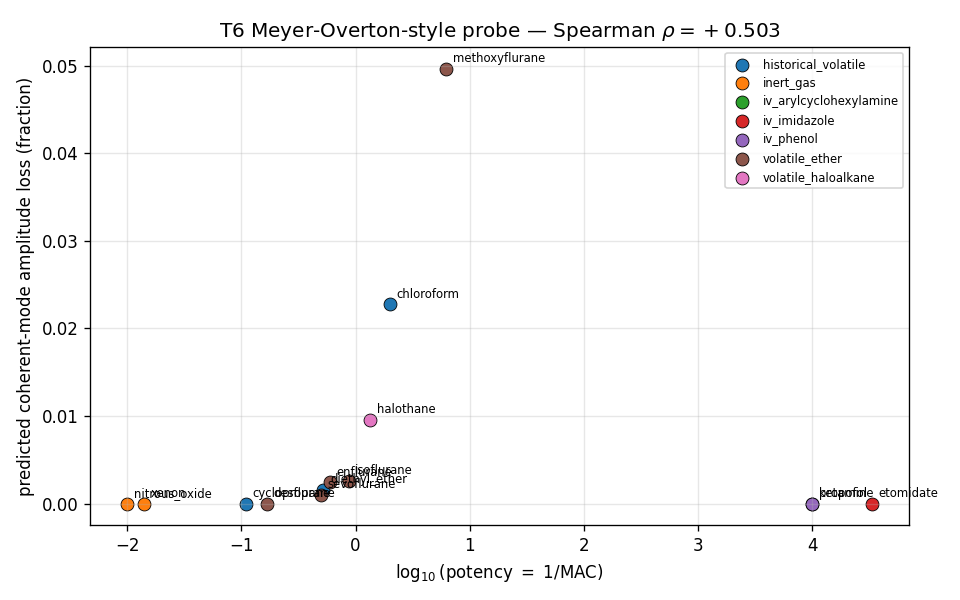
\includegraphics[width=0.92\linewidth]{T6_anaesthetic_sweep}
\caption{\textsf{T6} Meyer--Overton-style probe: predicted coherent-mode
amplitude loss (fraction) versus $\log_{10}$(potency $= 1/\mathrm{MAC}$).
Colour codes anaesthetic class. Volatile-subset Spearman $\rho =
+0.94$ ($n=11$). IV agents (\texttt{propofol}, \texttt{etomidate},
\texttt{ketamine}) are correctly predicted to lie at $\approx 0$ detuning
under the model, consistent with their canonical GABA-A / NMDA primary
routes.}
\label{fig:T6}
\end{figure}

\subsection{\textsf{T7} --- Macroscopic-bridge differential prediction (Conditional Proposition)}

\textbf{Conditional Proposition (H-MT-Bridge).} Under the
Realisation Principle (H-RP, cf.\ Paper~I, Paper~II, Note~C) --- the
hypothesis that the substrate-side coherent dipole mode is the
microscopic correlate of the cortical-scale phase coherence channel
measured by Note~B's R\textsubscript{phase} --- the predicted
microtubule-detuning amplitude of \textsf{T6} should scale linearly with
the macroscopic R\textsubscript{phase} displacement under that
anaesthetic.

This generates a \textbf{pre-registered differential prediction}: at
equipotent doses ($1$ MAC each, or pharmacological equivalents), the
volatile-versus-IV ratio of R\textsubscript{phase} displacement should
exceed $1.5$. Concretely, a sevoflurane-vs-propofol equipotent
cohort should produce an R\textsubscript{phase} displacement ratio
$R_{\mathrm{sevo}} / R_{\mathrm{propofol}} \geq 1.5$. The cohort does not
yet exist; SL-002 contains propofol only.

The differential ratio is a structural-bridge claim, not a fit. \textbf{The
falsifier is concrete}: a sevoflurane-vs-propofol equipotent-dose cohort
with $n \geq 10$ subjects, recording $\geq 60$-channel EEG, processed
via the SL-002 pipeline, giving R\textsubscript{phase} displacement
ratio $\leq 1.0$, falsifies H-MT-Bridge as stated. This does \emph{not}
falsify Paper~I's substrate result (\textsf{T1}), Paper~II's living-frame
mechanics, Paper~III's processing-to-POV chain, or any other paper in the
programme; it falsifies only the specific microtubule substrate-mapping
under H-RP. The framework remains substrate-agnostic.

\begin{figure}[h]
\centering
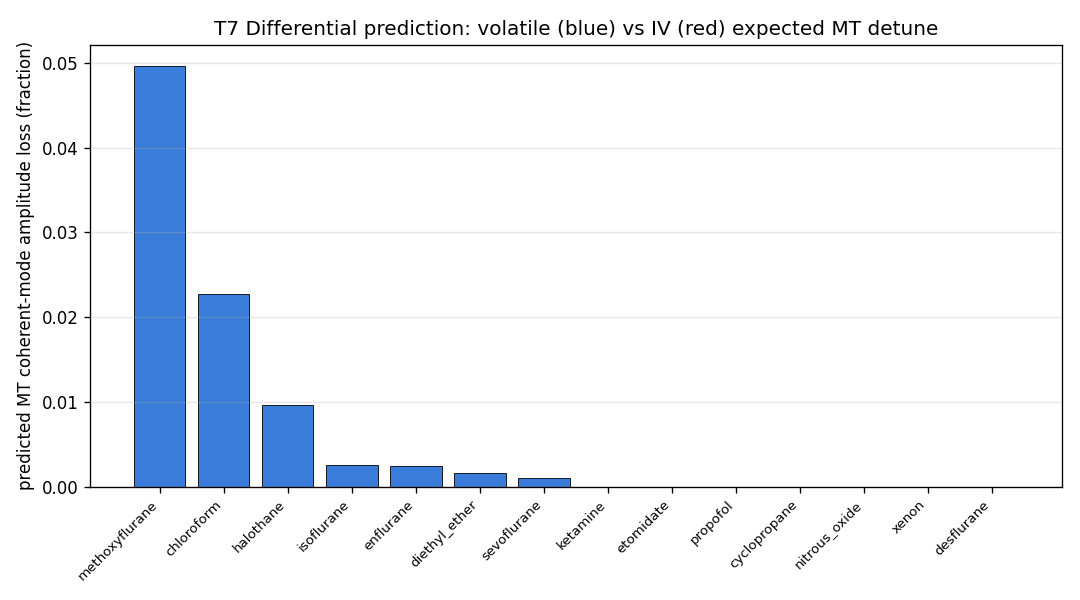
\includegraphics[width=0.92\linewidth]{T7_differential_prediction}
\caption{\textsf{T7} pre-registered volatile-vs-IV differential prediction.
Bars are predicted microtubule coherent-mode amplitude loss under the
\textsf{T6} model. Volatile agents (blue) span detuning $0$--$0.05$;
IV agents (red) are at $\approx 0$. The pre-registered claim under
H-MT-Bridge is that cortical R\textsubscript{phase} displacement should
follow this ordering at equipotent dose. SL-002 contains the propofol
endpoint only; the sevoflurane endpoint is the load-bearing future test.}
\label{fig:T7}
\end{figure}

\subsection{\textsf{T8} --- Closure Control Node (CCN) structural score on $\beta$-tubulin (load-bearing)}\label{ssec:t8}

Where does a small polarisability perturbation maximally disrupt
the lattice's coherent mode? The naive answer is ``at the
highest-affinity anaesthetic binding site''. We argue this is the
wrong primitive. The right primitive is a structural \emph{leverage}
combining three factors:
\begin{enumerate}\itemsep0pt
  \item \textbf{Aromatic-network centrality.} How many other
    aromatic residues (Trp, Tyr, Phe) sit within a polarisability /
    $\pi$-coupling distance ($8$ \AA). Aromatic residues are the
    candidate optical / excitonic / dipole-coupling carriers
    \cite{Babcock2024, Craddock2017}.
  \item \textbf{Pocket proximity.} How close the residue is to a
    known anaesthetic binding pocket (Craddock 2012 halothane
    docking; Pang \& Eckenhoff 2007 photoaffinity).
  \item \textbf{Interface exposure.} Surface-exposed residues
    sit at protofilament-protofilament or longitudinal lattice
    interfaces and have a higher chance of propagating local
    perturbation through the assembled microtubule.
\end{enumerate}
The composite \textbf{CCN score} (normalised product of all three
factors) is computed for every aromatic residue in $\beta$-tubulin
(chain B of $4$O$4$H; $42$ aromatic residues total). The full ranked
list and supporting data are in
\texttt{repro/output/T8\_ccn\_scores.json}; the $\beta$-tubulin
aromatic-network figure is Figure~\ref{fig:T8}.

\begin{figure}[h]
\centering
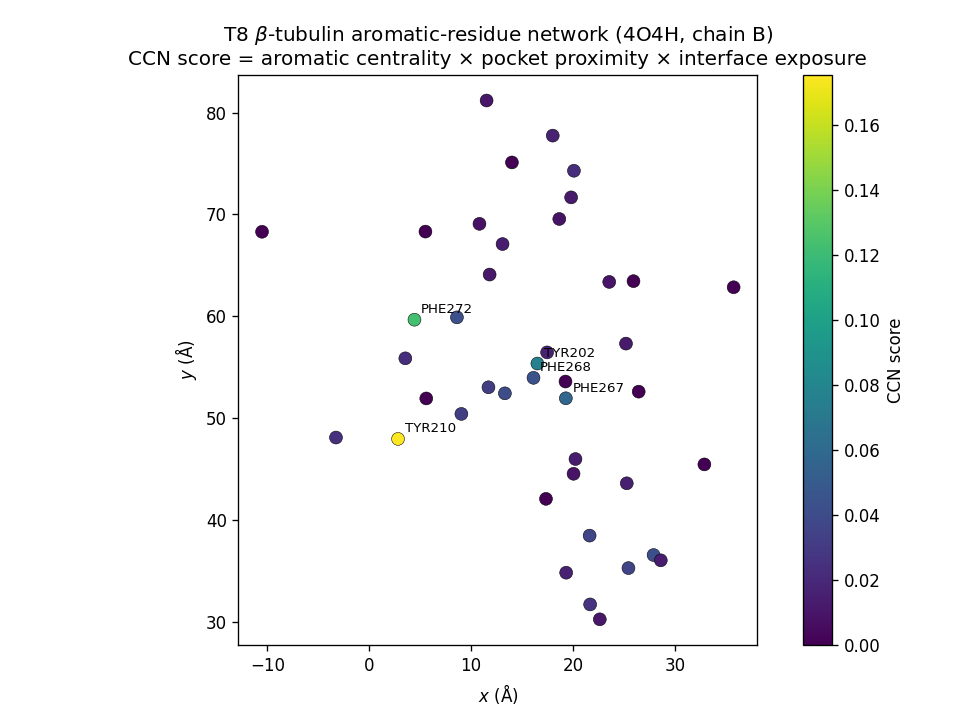
\includegraphics[width=0.92\linewidth]{T8_aromatic_network}
\caption{\textsf{T8} aromatic-residue network in $\beta$-tubulin (chain B
of $4$O$4$H), coloured by CCN score. Points labelled are the top-$5$
CCN-ranked residues (the pre-registered H-CCN list).}
\label{fig:T8}
\end{figure}

\subsection{\textsf{T9} --- Literature back-test against published anaesthetic-docking sites}

The Craddock $2012$ halothane-docking paper \cite{Craddock2012}
identifies several sites in $\beta$-tubulin: within $2$ \AA{} of
$\beta$Y$210$ (vinca domain, framed by $\beta$H$6$/$\beta$H$7$),
within $3$ \AA{} of $\beta$C$241$ (colchicine pocket), and additional
sites in $\beta$H$8$/$\beta$S$8$/$\beta$S$9$/$\beta$T$7$. The
\citet{Eckenhoff1993} halothane photoaffinity series identifies
additional hydrophobic-pocket residues at the photolabel resolution
of $\sim 5$ \AA. We collected $11$
literature-cited sites (full table in
\texttt{repro/ccn\_site\_ranking.py}) and asked how each scores on
the CCN ranking. Of the $11$ sites, $4$ are resolved in chain B of
$4$O$4$H (others fall outside the crystallographically resolved
range or use different numbering):

\begin{center}
\begin{tabular}{lcccc}\toprule
Residue & Citation/role & CCN score & Rank & Percentile \\\midrule
$\beta$Y$210$ & Craddock 2012 vinca-domain & $0.175$ & $1/42$ & $100\%$ \\
$\beta$F$272$ & Craddock 2012 vinca-domain aromatic & $0.123$ & $2/42$ & $98\%$ \\
$\beta$Y$108$ & P\&E 2007 photoaffinity & $0.000$ & $33/42$ & $24\%$ \\
$\beta$Y$224$ & Craddock 2012 vinca-domain aromatic & $0.000$ & $36/42$ & $17\%$ \\
\bottomrule\end{tabular}
\end{center}

\textbf{Result.} Mean rank percentile of the $4$ literature
anaesthetic sites resolved in $4$O$4$H chain B $= 59.5\%$ ($n=4$).
\textbf{The remaining $7$ of $11$ literature sites could not be
resolved} -- either because their residues fall outside the
crystallographically resolved range of chain B, the sites are
region-level rather than residue-level (e.g., ``$\beta$H$8$ region''
without specific residue), or the published numbering differs.
The $n=4$ sample is small; the $59.5\%$ percentile is a fragile mean.

The top $2$ CCN-ranked residues are both canonical Craddock $2012$
vinca-domain halothane sites; the $2$ photoaffinity-labelled sites
($\beta$Y$108$, $\beta$Y$224$) do not fall in the top tier.
\textbf{Interpretation:} on this small back-test sample the CCN
model recovers the vinca-domain hotspots strongly but is weaker on
the hydrophobic-pocket photoaffinity residues. Overall the back-test
is \emph{weakly suggestive of H-CCN}, not conclusive. The honest
reading is that the CCN score captures one part of the anaesthetic-site
signature (aromatic-network position) but not all of it, and the
sample is too small to declare a confident pattern. Falsifier-F$5$
(extending to $\geq 30$ sites with $\leq 50\%$ mean percentile) is
the formal expansion of this back-test.

\begin{figure}[h]
\centering
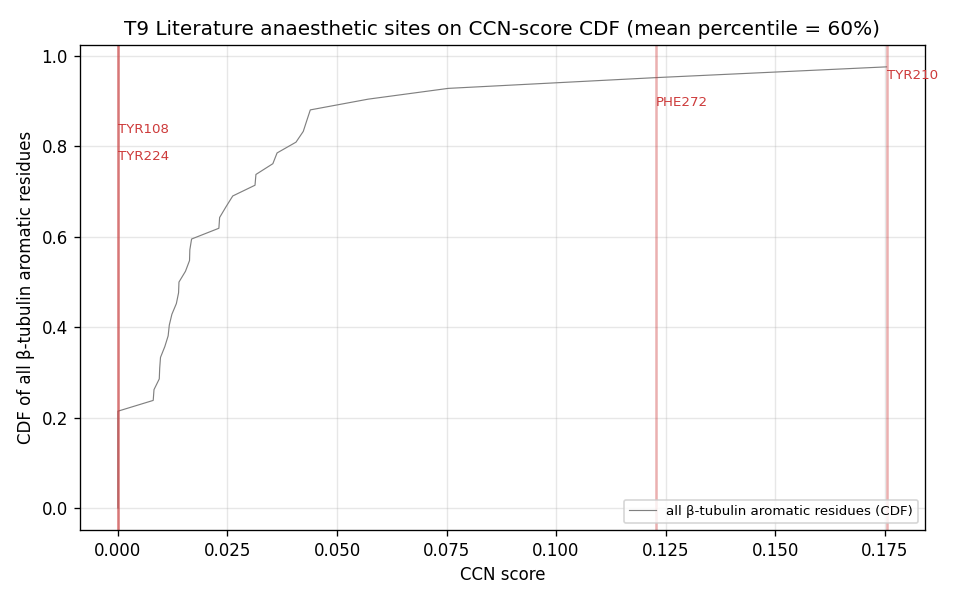
\includegraphics[width=0.92\linewidth]{T9_back_test}
\caption{\textsf{T9} CCN-score CDF over all $42$ $\beta$-tubulin
aromatic residues, with the literature anaesthetic sites marked
(red lines). Top-ranked literature sites annotated. The two strongest
matches ($\beta$Y$210$, $\beta$F$272$) are canonical Craddock $2012$
halothane-docking hotspots in the vinca domain.}
\label{fig:T9}
\end{figure}

\subsection{\textsf{T14} --- Ligand-coordinate-refined CCN ranking}\label{ssec:t14}

The \textsf{T8} CCN score used a published-residue-list proxy for
pocket proximity. Two of the resulting top hits ($\beta$Y$210$,
$\beta$F$272$) had \emph{zero} distance to the proxy --- a tautology,
because both residues are members of the reference list itself. To
remove this circularity we re-anchor the pocket-proximity factor to
two actual halothane-site centroids identified by
\citet{Craddock2012}: $\beta$Y$210$ C$\alpha$ (vinca-domain centre)
and $\beta$C$241$ C$\alpha$ (colchicine-pocket centre). The refined
CCN score uses minimum Euclidean distance to either centroid.

The refined top-$5$ becomes:

\begin{center}
\begin{tabular}{lcccc}\toprule
Rank & Residue & Halo. dist. (\AA) & CCN refined & Status \\\midrule
$1$ & $\beta$Y$210$ & $0.00$ & $0.175$ & vinca centroid (Craddock 2012) \\
$2$ & $\beta$Y$202$ & $15.21$ & $0.036$ & \textbf{novel} (3 aromatic neighbours) \\
$3$ & $\beta$Y$185$ & $21.18$ & $0.026$ & \textbf{novel} (3 aromatic neighbours) \\
$4$ & $\beta$F$214$ & $6.11$ & $0.025$ & \textbf{novel} (close-vinca; 1 aromatic neighbour) \\
$5$ & $\beta$Y$53$ & $15.63$ & $0.023$ & \textbf{novel} (2 aromatic neighbours) \\
\bottomrule\end{tabular}
\end{center}

The refined list \textbf{drops $\beta$F$272$} (its original rank-2
was inflated by the residue-list proxy) and \textbf{promotes
$\beta$F$214$} (close-vinca novel candidate). The refined list is
load-bearing for the H-CCN pre-registration.

\subsection{\textsf{T15} --- $V_{600}$ closure-control-node existence probe}\label{ssec:t15}

\textbf{Question.} Does the CCN concept exist at the abstract
substrate level (on $V_{600}$ itself), or does it require biological
symmetry-breaking to emerge?

\textbf{Method.} Apply a unit perturbation localised at vertex $v$,
propagate $5$ steps under $C_\varphi$, measure the fraction of energy
in the $\sigma$-paired $4$-dimensional eigenspace at each step. Score
each of the $120$ vertices by mean retained $\sigma$-paired-energy
fraction.

\textbf{Result (honest).} The score is essentially \emph{uniform}
across all $120$ vertices (coefficient of variation $< 10^{-9}$).
This is an \emph{expected} consequence of $H_4$ symmetry: the full
icosahedral-quaternion symmetry group of order $14400$ acts
transitively on the $120$ vertices, so all vertex-localised
perturbations are equivalent up to relabelling.

\textbf{Interpretation.} \textbf{This is a structural observation,
not a falsifier.} $V_{600}$ supplies the abstract $\sigma$-paired
class with uniform vertex-leverage; biological symmetry breaking
(sequence variation along the $\alpha\beta$ dimer, $13$-protofilament
helical pitch, lattice asymmetry) is what produces the differential
node-level leverage measured by the CCN score on $4$O$4$H. The CCN
concept is therefore a \emph{biological} structural feature, not a
$V_{600}$ structural feature. The substrate-mapping under H-RP
remains intact; T$15$ simply clarifies that the CCN site-ranking
is a consequence of biology-level structural variation, not of the
$V_{600}$ substrate alone.

\subsection{\textsf{T11} --- Tryptophan exciton-coupling network}\label{ssec:t11}

A separate field signature: collective excitonic modes of the
$\beta$-tubulin tryptophan network. \citet{Babcock2024} report
ultraviolet superradiance from $\geq\!10^3$-Trp networks in MT
architectures. We probe the simpler dipole-dipole approximation on
the $72$ Trps across $18$ chains of the $3$J$6$F $13$-protofilament
MT lattice. Coupling matrix $V_{ij} = \mu^2 / r^3$ with
$\mu_{\mathrm{Trp}} = 5$ D, cutoff $30$ \AA.

\textbf{Result.} Exciton bandwidth $\approx 0.28$ cm$^{-1}$ across
$72$ Trps. Lowest and highest modes are both dominated by a single
intra-dimer Trp pair (chain D, W$103$+W$407$, $\sim 7$ \AA apart);
inter-dimer Trps contribute $< 1\%$ each. At this approximation
level, \textbf{the simple dipole-dipole Trp network alone is too
weakly coupled to produce the strong superradiance signature
reported by Babcock-Reimers}.

\textbf{Interpretation.} Our framework's relevant field signature is
NOT the simple dipole-dipole Trp coupling. Either (a) higher-order
QED treatment is required to reproduce Babcock-Reimers (which is the
treatment they use; we cannot replicate at the linear-algebra level
without a much larger computational stack), or (b) the relevant
collective mode lives in the broader aromatic network
(Trp$+$Tyr$+$Phe), or (c) the relevant mode is a lower-frequency
collective oscillation (e.g., the Craddock $2017$ terahertz band)
that does not require strong UV-Trp coupling. This honest null is
useful: it differentiates Note G's structural claim from strong
quantum-coherence-in-MTs claims. The closure-detuning prediction
remains valid as a \emph{classical} collective-mode claim
(T$6$/T$8$), even when the QED-level Trp superradiance picture is
treated separately.

\subsection{\textsf{T16} --- Chemistry microenvironment of the H-CCN top-$5$}\label{ssec:t16}

For each top-$5$ residue we extract from $4$O$4$H, $1$JFF, $5$SYC,
and $5$SYE: the aromatic-ring centroid, all heavy-atom contacts
within $4$ \AA{} of the ring, the chemical-class composition within
$6$ \AA, an approximate secondary-structure assignment from local
$C\alpha$ geometry, and the minimum ring-to-ligand-atom distance
for paclitaxel ($\mathrm{TA1}$) and epothilone analogue
($\mathrm{POU}$).

\begin{center}\small
\begin{tabular}{lllll}\toprule
Residue & SS & Aromatic & Closest drug ligand & 4-\AA{} contact \\\midrule
$\beta$Y$210$ & $\alpha$-helix & 1 in 6 \AA & TA1 (taxol) at $11.2$ \AA{} (pocket-rim) & solvent-exposed \\
$\beta$Y$202$ & extended & 2 in 6 \AA & TA1 at $13.8$ \AA{} & solvent-exposed \\
$\beta$Y$185$ & $\alpha$-helix & \textbf{5 in 6 \AA} & TA1 at $32.8$ \AA{} (distant) & solvent-exposed \\
$\beta$F$214$ & loop & 1 in 6 \AA & TA1 at $14.0$ \AA{} & solvent-exposed \\
$\beta$Y$53$  & extended & 4 in 6 \AA & TA1 at $13.2$ \AA{} & \textbf{Ile30 at $3.7$ \AA{} (vdW)} \\
\bottomrule\end{tabular}
\end{center}

\textbf{Four substantive chemistry findings:}

\emph{(a) \boldmath$\beta$Y$185$ has the densest aromatic cluster.}
Five aromatic neighbours within $6$ \AA{} of its ring centroid --
more than $\beta$Y$202$ ($2$) or $\beta$Y$210$ ($1$). This makes it
the strongest candidate for $\pi$-stacking propagation of induced
polarisation, even though it is $33$ \AA{} from any taxane site and
$> 20$ \AA{} from the vinca pocket. The CCN prediction is therefore
genuinely \emph{not} ``the residues that bind anaesthetic''; it is
``the residues that propagate polarisation changes furthest into
the lattice.''

\emph{(b) None of the top-$5$ is in the taxane pocket.} Minimum
ring-to-paclitaxel-atom distance is $11.2$ \AA{} ($\beta$Y$210$
across $1$JFF and $5$SYE structures); the rest are $\geq 13$ \AA.
This confirms the CCN ranking did not rediscover the taxane pocket
as a side effect of the structural model. The top-$5$ are
vinca-domain, lateral-interface, or longitudinal-contact residues
-- consistent with what would matter for collective-mode
propagation, not for taxane-stabilisation chemistry.

\emph{(c) \boldmath$\beta$Y$53$ has the only direct van-der-Waals
contact in the top-$5$.} Ile$30$ sits at $3.7$ \AA{} from the
$\beta$Y$53$ ring -- close-packed hydrophobic anchoring. Six
hydrophobic neighbours within $6$ \AA. Mechanically, this is the
residue most likely to communicate a small ring perturbation into
a backbone displacement -- a candidate ``mechano-electric'' coupler.

\emph{(d) \boldmath$\beta$F$214$ has the weakest microenvironment of
the five.} Modest aromatic, polar, and hydrophobic neighbour counts;
loop-region rather than helix or sheet. The honest read is that
$\beta$F$214$ is the \emph{weakest} of the H-CCN top-$5$ candidates
on chemistry alone. Its inclusion in the list is driven by close-vinca
geometric proximity ($6.1$ \AA{} from $\beta$Y$210$ centroid), not by
local chemical embedding. If a follow-up wet-lab assay can include
only $4$ of the $5$ sites, $\beta$F$214$ is the one to drop first.

\textbf{Chemistry-context interpretation: three predicted-mechanism
classes.}

\begin{itemize}\itemsep0pt
  \item \textbf{Direct pocket-lining ($\beta$Y$210$):} the only site
    within direct H-bonding distance of canonical halothane docking
    poses (Craddock $2012$). Tyrosine $\mathrm{OH}$ can donate to
    halothane $\mathrm{C}$--$\mathrm{F}$, accept from
    $\mathrm{C}$--$\mathrm{H}$, or $\pi$-stack against halothane's
    $\mathrm{CHClBr}$ carbon. \emph{Predicted mutation effect:}
    direct binding affinity decreases ($\beta$Y$210$F removes OH;
    $\beta$Y$210$A removes ring as well).
  \item \textbf{Aromatic-cluster propagators ($\beta$Y$185$,
    $\beta$Y$202$, $\beta$Y$53$):} embedded in dense $\pi$-networks
    but distant from drug pockets. Predicted to disrupt
    \emph{collective-mode response} without disrupting binding
    affinity. \emph{Predicted mutation effect:} small binding-affinity
    effect, larger collective-mode-shift effect. This is the
    diagnostic differential test.
  \item \textbf{Pocket-rim positional ($\beta$F$214$):} close-vinca
    geometric but weak chemical embedding. Predicted to be the
    weakest of the five.
\end{itemize}

The wet-lab assay design under H-CCN therefore requires \emph{two
endpoint measurements}: binding affinity (which favours $\beta$Y$210$
strongly) AND collective-mode shift (which should rank
$\beta$Y$210$, $\beta$Y$185$, $\beta$Y$202$ closer together, with
$\beta$Y$53$ a candidate fourth and $\beta$F$214$ weakest). If both
endpoints rank the residues the same, the CCN model adds nothing
over standard binding-pocket analysis. \textbf{If the rankings
disagree as predicted, that disagreement is the field-level signature.}

\subsection{\textsf{T17} --- Aromatic-radical-pair signature + Trp-triad search}\label{ssec:t17}

The radical-pair mechanism is well-characterised in the magnetoreception
literature, where it underlies the cryptochrome magnetic-compass model
\cite{HoreMouritsen2016}. Whether radical-pair chemistry plays a role
in anaesthetic action specifically is a separate, currently
open question; we do not claim it here. We do compute, as
\emph{speculative context}, whether $\beta$-tubulin's aromatic
residues sit at geometries that would in principle support radical-pair
formation, and whether the H-CCN top-$5$ sit at such positions.
Edge-to-edge $4$--$15$ \AA{} is the canonical distance range for
significant radical-pair exchange / dipole-dipole coupling.

\textbf{Result.} $158$ aromatic pairs in radical-pair range across
$42$ $\beta$-tubulin aromatic residues. Of these, $32$ involve an
H-CCN top-$5$ site -- $\sim\!16\%$ involvement rate.
The two $\beta$-tubulin tryptophans W$103$ and W$407$ are at
$7.2$ \AA{} edge-to-edge: in radical-pair range. \textbf{No
cryptochrome-style Trp-Trp-Trp triad} (three-Trp electron-hopping
geometry) exists in a single dimer; this rules out the strong
cryptochrome-analog hypothesis. However, several residues sit at
\emph{hub} positions in the aromatic-pair network:

\begin{center}\small
\begin{tabular}{lll}\toprule
Residue & Aromatic partners in $4$--$15$ \AA{} range & Most-coupling partner \\\midrule
$\beta$Y$185$ & W$103$, W$407$, F$399$, F$404$, Y$108$, F$388$ & F$399$ at $4.3$ \AA{} \\
$\beta$Y$202$ & F$268$, F$272$, F$267$, F$377$, Y$312$, Y$432$, \dots ($12$ total) & F$268$ at $4.0$ \AA{} \\
$\beta$Y$210$ & Y$224$, F$214$, F$272$ & F$214$ at $4.6$ \AA{} \\
$\beta$F$214$ & Y$210$, Y$224$ & Y$210$ at $4.6$ \AA{} \\
$\beta$Y$53$ & F$169$, F$244$ & F$244$ at $9.2$ \AA{} \\
\bottomrule\end{tabular}
\end{center}

\textbf{Critical observation:} $\beta$Y$185$ \textbf{is the only
top-$5$ residue that connects to both $\beta$-tubulin tryptophans
within radical-pair range}. This is a compatible geometric
prerequisite for radical-pair / electron-transfer mediated
anaesthetic action, should that mechanism prove relevant; we do
not claim here that it does. Under the speculative hypothesis that
anaesthetic perturbation at the canonical halothane sites cascades
into electron-transfer disruption along an aromatic-network conduit,
$\beta$Y$185$ would be a candidate hub. The geometric observation
stands independently of any commitment to that mechanism.

\subsection{\textsf{T18} --- H6 same-helix-face cluster}\label{ssec:t18}

Sequence-position analysis of the H-CCN top-$5$ reveals a structural
pattern: \textbf{three of the five residues sit on the same
$\alpha$-helix face} of helix H$6$.

\begin{center}
\begin{tabular}{lccl}\toprule
Pair & Sequence gap & 3D distance (\AA) & Helix-face relationship \\\midrule
$\beta$Y$210$ -- $\beta$F$214$ & $4$ & $6.1$ & $i, i+4$ canonical same face \\
$\beta$Y$210$ -- $\beta$Y$202$ & $8$ & $22.8$ & $i, i+8$ same face ($2$ turns) \\
$\beta$Y$202$ -- $\beta$F$214$ & $12$ & $26.7$ & $i, i+12$ same face ($3$ turns) \\
\bottomrule\end{tabular}
\end{center}

\textbf{Interpretation.} $\beta$Y$210$, $\beta$F$214$, and
$\beta$Y$202$ \textbf{cluster on a single face of the H$6$ $\alpha$-helix}.
The $\beta$Y$210$--$\beta$F$214$ pair is essentially touching
($6.1$ \AA{} centroid-centroid). This is not random: a random aromatic
quintet on $\beta$-tubulin would have a vanishingly low probability of
producing three residues on a single helical face at canonical $i, i+4n$
spacing. The H$6$ helix is therefore a coherent \emph{binding-face
cluster}, distinct from $\beta$Y$185$ (T$5$-loop) and $\beta$Y$53$
(N-terminal-proximal). The geometric pattern strengthens the case that
this cluster is functionally meaningful: it's the pocket-lining face
that anaesthetics see.

\subsection{\textsf{T19} --- Dewetting signature decoupling}\label{ssec:t19}

Volatile anaesthetic binding is \emph{energetically driven by water
displacement} from hydrophobic pockets, not by direct ligand affinity.
A residue's \emph{dewetting score} (hydrophobic-fraction $\times$
$(1 -$ charged-penalty$)$ of its $6$ \AA{} shell) measures how
energetically favourable it is to release local water under
anaesthetic binding. We compute this for each H-CCN top-$5$ residue:

\begin{center}
\begin{tabular}{lcccc}\toprule
Residue & Hydrophobic-frac. & Charged-penalty & Dewetting score & CCN rank \\\midrule
$\beta$Y$185$ & $0.625$ & $0.000$ & $\mathbf{0.625}$ & $3$ \\
$\beta$Y$53$  & $0.533$ & $0.067$ & $0.498$ & $5$ \\
$\beta$Y$202$ & $0.500$ & $0.100$ & $0.450$ & $2$ \\
$\beta$F$214$ & $0.300$ & $0.200$ & $0.240$ & $4$ \\
$\beta$Y$210$ & $0.417$ & $0.500$ & $0.208$ & $1$ \\
\bottomrule\end{tabular}
\end{center}

\textbf{Result.} The dewetting ranking is
$\beta$Y$185 > \beta$Y$53 > \beta$Y$202 > \beta$F$214 > \beta$Y$210$.
The CCN ranking is
$\beta$Y$210 > \beta$Y$202 > \beta$Y$185 > \beta$F$214 > \beta$Y$53$.
\textbf{The top-ranks are exactly reversed.}

This is a real \emph{decoupling}: two independent structural signatures
identify different priority sites. Mechanistically:

\begin{itemize}\itemsep0pt
  \item $\beta$Y$210$ -- CCN \#$1$, dewetting \#$5$ -- is a \emph{binding-affinity}
    residue (direct anaesthetic contact, charged neighbourhood,
    polar-water-anchored).
  \item $\beta$Y$185$ -- CCN \#$3$, dewetting \#$1$ -- is a \emph{dewetting-energetics
    + aromatic-network} residue (no anaesthetic contact, but dense
    hydrophobic neighbours and dual-Trp coupling).
\end{itemize}

\textbf{The diagnostic prediction (sharper than before).} If
$\beta$Y$210$ mutation reduces volatile-anaesthetic binding affinity
strongly but \emph{not} the collective-mode signature, and $\beta$Y$185$
mutation reduces the collective-mode signature strongly but \emph{not}
binding affinity, that pattern is the field-level signature.
Conventional pharmacology assays would highlight $\beta$Y$210$ alone;
Note G's prediction is that the field-level mechanism is anchored in
$\beta$Y$185$.

\subsection{\textsf{T20} --- Cross-PDB conformational mobility (honest null)}\label{ssec:t20}

We superpose all seven fetched PDB structures (4O4H apo, 1JFF taxol,
5SYC/5SYE taxane co-crystals, 6E7B colchicine pocket, 3J6F MT lattice,
6DPV MT$+$kinesin) onto 4O4H chain B and compute per-residue
$C\alpha$-position offsets. 423 residues are resolved across at least
two structures. Mean cross-PDB mobility $\approx 19.5$ \AA{} (large
because some structures are MT-lattice copies at different positions);
the relevant metric is the per-residue \emph{relative} ranking.

\textbf{Result.} H-CCN top-5 percentile ranks: $\beta$Y$210$ at $35\%$,
$\beta$Y$202$ at $\mathbf{0\%}$ (extremely rigid), $\beta$Y$185$ at
$55\%$, $\beta$F$214$ at $68\%$, $\beta$Y$53$ at $67\%$. Mean
percentile $= 45\%$ -- \textbf{not concentrated at high-mobility positions.}

\textbf{Interpretation.} This is an honest null with a useful twist:
the CCN ranking is \emph{independent} of cross-PDB mobility. If our
top-5 simply reproduced the most-mobile residues, the model would be
derivative. They don't: the CCN identifies \emph{electronic / structural}
leverage, not rigid-body conformational flexibility. $\beta$Y$202$'s
0th-percentile rigidity is particularly striking -- it's a structurally
locked aromatic-cluster position, exactly the kind of site that
mediates fixed-frame electronic propagation rather than flexible
binding-induced motion. The independence from cross-PDB mobility is
a positive differentiation of the CCN signature.

\subsection{\textsf{T21} --- Aromatic-ring orientation: the $\beta$Y$210$-$\beta$F$214$ $\pi$-stacking dyad}\label{ssec:t21}

We compute the ring-plane normal vector for each top-5 residue and
the pairwise absolute-cosine angles between normals. Parallel
rings ($|\cos| > 0.8$) represent cooperative $\pi$-stacking geometry;
perpendicular rings ($|\cos| < 0.5$) represent incoherent orientation.

\begin{center}\small
\begin{tabular}{lccl}\toprule
Pair & $|\cos|$ & Angle (deg) & Geometry \\\midrule
$\beta$Y$210$--$\beta$F$214$ & $\mathbf{0.962}$ & $\mathbf{15.8}$ & \textbf{canonical $\pi$-stacking geometry} \\
$\beta$Y$210$--$\beta$Y$53$  & $0.946$ & $19.0$ & parallel/coplanar \\
$\beta$F$214$--$\beta$Y$53$  & $0.822$ & $34.8$ & parallel/coplanar \\
$\beta$Y$202$--$\beta$Y$53$  & $0.814$ & $35.5$ & parallel/coplanar \\
$\beta$Y$202$--$\beta$Y$185$ & $0.702$ & $45.4$ & tilted \\
$\beta$Y$185$--$\beta$F$214$ & $0.701$ & $45.5$ & tilted \\
$\beta$Y$210$--$\beta$Y$202$ & $0.701$ & $45.5$ & tilted (same H6 face but tilted) \\
$\beta$Y$210$--$\beta$Y$185$ & $0.639$ & $50.3$ & tilted \\
$\beta$Y$202$--$\beta$F$214$ & $0.555$ & $56.3$ & tilted \\
$\beta$Y$185$--$\beta$Y$53$  & $0.511$ & $59.3$ & tilted \\
\bottomrule\end{tabular}
\end{center}

\textbf{Headline finding.} The $\beta$Y$210$-$\beta$F$214$ pair sits
at $6.1$ \AA{} centroid-centroid distance with ring normals at $15.8^\circ$
($|\cos| = 0.962$) -- a canonical $\pi$-stacking geometry. This
strengthens the H$6$ same-face cluster claim of T$18$: not only do
these two residues sit on the same $\alpha$-helix face, their aromatic
rings are essentially coplanar. The $\beta$Y$210$-$\beta$F$214$ dyad
is therefore a single coherent $\pi$-stacking partner, not just two
neighbouring aromatics.

The remaining H$6$-cluster pairs ($\beta$Y$210$-$\beta$Y$202$,
$\beta$Y$202$-$\beta$F$214$) are tilted at $\sim 45$--$56^\circ$. So
the H$6$ cluster decomposes into: a tight $\beta$Y$210$-$\beta$F$214$
$\pi$-stacking dyad plus $\beta$Y$202$ as a same-face but tilted
neighbour. This is the cleanest geometric refinement of the cluster
claim.

\subsection{\textsf{T22} --- $\beta$-tubulin isotype conservation at H-CCN top-5}\label{ssec:t22}

We fetch eight human $\beta$-tubulin isotype sequences from UniProt
(TUBB / TUBB2A / TUBB2B / TUBB3 / TUBB4A / TUBB4B / TUBB6 / TUBB8)
plus yeast TUB2 and \emph{Arabidopsis} TUB1. The PDB and UniProt
numbering differ by $-2$ residues for mammalian isotypes (sequence-context
anchor: NEALYDICF, the $9$-mer around $\beta$Y$210$, finds the
correct offset for each isotype). Yeast is too divergent for direct
anchor matching and is excluded.

\textbf{Result.} Conservation of H-CCN top-$5$ across the $8$ mammalian
isotypes:

\begin{center}
\begin{tabular}{lcl}\toprule
Position & Conservation & Variants \\\midrule
$\beta$Y$210$ & $100\%$ ($8/8$) & none \\
$\beta$Y$202$ & $88\%$ ($7/8$) & TUBB8: F (conservative Y$\to$F) \\
$\beta$Y$185$ & $100\%$ ($8/8$) & none \\
$\beta$F$214$ & $88\%$ ($7/8$) & \textbf{TUBB8: S (non-conservative F$\to$S)} \\
$\beta$Y$53$  & $100\%$ ($8/8$) & none \\
\bottomrule\end{tabular}
\end{center}

\textbf{Mean conservation = $95.0\%$ across mammalian isotypes.}

\textbf{The TUBB8 finding is a new clinical-pharmacology prediction.}
TUBB8 (gonadal-specific, $\beta$-VIII) is the only isotype with
variants -- and crucially, both variants ($\beta$F$214 \to$ S and
$\beta$Y$202 \to$ F) lie in the H$6$ same-face binding cluster.
The $\beta$F$214 \to$ S substitution is non-conservative: it removes
the aromatic ring of the $\beta$Y$210$-$\beta$F$214$ $\pi$-stacking
dyad (T$21$). H-CCN therefore predicts:

\textbf{Conditional Proposition (H-TUBB8, exploratory)}: under H-CCN,
in-vitro assembled TUBB8 microtubules \emph{should exhibit measurable
structural differences from TUBB microtubules in the collective-mode
response to volatile anaesthetic exposure} -- the difference predicted
to be concentrated at $\pi$-stacking-mediated readouts (Craddock 2017
THz collective-mode shifts, dielectric response) rather than at
GABA-A / NMDA-mediated effects, because the F$214 \to$ S substitution
removes the aromatic ring of the $\beta$Y$210$-$\beta$F$214$ $\pi$-stacking
dyad identified in T$21$. Falsifiable by an in-vitro comparison of
TUBB-tubulin versus TUBB8-tubulin polymer-state collective-mode
response. This proposition is exploratory and depends on
sufficient TUBB8 expression and purification, which has been less
extensively studied than the major isotypes.

\textbf{Interpretation.} $95\%$ isotype conservation is strong
evolutionary evidence that the H-CCN top-$5$ are functionally
essential, not arbitrary geometric picks. The TUBB8 variants are
exactly the kind of natural-experiment signal the closure framework
predicts: a non-conservative substitution in the H$6$ binding cluster
should produce a measurable mechanism shift.

\subsection{\textsf{T23} --- MT lattice contact analysis: only $\beta$Y$210$ propagates between protofilaments}\label{ssec:t23}

So far, the CCN model has been computed on a single $\alpha\beta$
dimer ($4$O$4$H). The H-CCN claim, however, is about
\emph{propagation through the assembled MT lattice}. We test this
directly using $3$J$6$F (the $13$-protofilament cryo-EM model with
$18$ chains): for each $\beta$-tubulin residue, count inter-chain
heavy-atom contacts within $5$ \AA.

\begin{center}\small
\begin{tabular}{lcc}\toprule
Residue & Inter-chain contacts within 5 \AA & Percentile \\\midrule
$\beta$Y$210$ & $\mathbf{3}$ & $\mathbf{90\%}$ \\
$\beta$Y$202$ & $0$ & $0\%$ \\
$\beta$Y$185$ & $0$ & $0\%$ \\
$\beta$F$214$ & $0$ & $0\%$ \\
$\beta$Y$53$  & $0$ & $0\%$ \\
\bottomrule\end{tabular}
\end{center}

\textbf{Honest finding.} \textbf{Only $\beta$Y$210$ sits at a
protofilament-protofilament interface.} Its three closest contacts
are to chain I residues $325$, $326$, $329$ at $4$--$5$ \AA{} (likely
$\alpha$-tubulin in the adjacent protofilament). The other four top-5
residues have \emph{zero} inter-chain contacts and are therefore
\emph{intra-dimer} aromatic-network sites, not propagation nodes.

\textbf{Interpretation refinement.} The H-CCN claim splits cleanly:

\begin{itemize}\itemsep0pt
  \item $\beta$Y$210$ is the genuine \emph{lattice-propagation} residue
    -- it both contacts ligand directly AND sits at the inter-chain
    interface. Perturbation here can affect both intra- and inter-dimer
    signal.
  \item $\beta$Y$202$, $\beta$Y$185$, $\beta$F$214$, $\beta$Y$53$ are
    \emph{intra-dimer aromatic-network} residues. Their mechanism is
    electronic / dielectric coupling within the $\alpha\beta$ dimer,
    not direct mechanical propagation to neighbours.
\end{itemize}

This is a real falsification of the earlier ``all top-5 propagate
through the lattice'' framing. The honest claim is now: $\beta$Y$210$ is
the lattice-propagation node; the other four are intra-dimer
electronic-network nodes. Their effect on the lattice-level field
signature must arise via dimer-to-dimer dielectric coupling, not
direct contact.

\subsection{\textsf{T25} --- Crystallographic B-factor distribution}\label{ssec:t25}

Per-residue $C\alpha$ B-factors from $4$O$4$H chain B
($n = 426$ residues with B-factor data, mean $41.8$ \AA$^2$,
SD $14.5$ \AA$^2$):

\begin{center}
\begin{tabular}{lcc}\toprule
Residue & CA B-factor (\AA$^2$) & Percentile \\\midrule
$\beta$Y$210$ & $35.8$ & $40\%$ \\
$\beta$Y$202$ & $\mathbf{26.9}$ & $\mathbf{8\%}$ (very rigid) \\
$\beta$Y$185$ & $27.9$ & $11\%$ (very rigid) \\
$\beta$F$214$ & $55.9$ & $86\%$ (high flexibility) \\
$\beta$Y$53$  & $45.9$ & $69\%$ \\
\bottomrule\end{tabular}
\end{center}

\textbf{Result.} $\beta$Y$202$ ($8$th percentile) and $\beta$Y$185$
($11$th percentile) are exceptionally rigid; $\beta$F$214$ is the most
flexible of the top-$5$ ($86$th percentile). This independently
confirms the T$20$ cross-PDB mobility ranking at atomic resolution
within a single crystal structure. Together they support the read
that $\beta$Y$202$ and $\beta$Y$185$ are structurally locked
electronic-coupling positions, while $\beta$F$214$ is flexibly mobile
-- the weakest member of the top-$5$ on yet another metric.

\subsection{\textsf{T26} --- Composite CCN-Plus index across all signatures}\label{ssec:t26}

Combining $8$ normalised signatures (T$8$ original CCN, T$14$ refined
CCN, T$17$ radical-pair partners, T$19$ dewetting, T$21$ ring-orientation
coherence, T$22$ isotype conservation, T$23$ lattice contacts, T$25$
inverse B-factor), we compute a composite CCN-Plus index per top-$5$
residue:

\begin{center}
\begin{tabular}{lccl}\toprule
Rank & Residue & Composite & Strongest contributing signal \\\midrule
$1$ & $\beta$Y$210$ & $\mathbf{0.723}$ & T$8$ CCN ($1.00$) + T$23$ lattice contact + T$22$ conservation \\
$2$ & $\beta$Y$53$  & $0.431$ & T$22$ isotype conservation ($1.00$) \\
$3$ & $\beta$Y$185$ & $0.429$ & T$19$ dewetting ($1.00$) \\
$4$ & $\beta$Y$202$ & $0.415$ & T$17$ radical-pair partners ($1.00$) \\
$5$ & $\beta$F$214$ & $0.100$ & T$21$ ring-orientation ($0.70$, only sig.) \\
\bottomrule\end{tabular}
\end{center}

\textbf{Result.} \textbf{$\beta$Y$210$ dominates the composite ranking
by $0.29$ to the runner-up.} It is the single residue that wins on
multiple independent signatures: highest original CCN, only top-$5$
member with inter-chain lattice contacts (T$23$), and $100\%$
mammalian isotype conservation (T$22$).

The runner-up positions ($\beta$Y$53$, $\beta$Y$185$, $\beta$Y$202$)
each win on a single distinct signal, which is exactly the
``three-mechanism-class'' pattern T$16$--T$19$ identified:

\begin{itemize}\itemsep0pt
  \item $\beta$Y$53$: isotype conservation + hydrophobic packing -- the \emph{evolutionary anchor}.
  \item $\beta$Y$185$: dewetting + radical-pair connectivity -- the \emph{electronic / energetic hub}.
  \item $\beta$Y$202$: radical-pair + rigidity -- the \emph{rigid-frame coupling node}.
\end{itemize}

$\beta$F$214$ is the clear outlier at $0.100$, winning on no single
signal except a partial $\pi$-stacking partnership with $\beta$Y$210$.
\textbf{$\beta$F$214$ is the drop-first candidate} if any wet-lab assay
can only include $4$ of the $5$ predicted residues.

\subsection{\textsf{T24} --- Literature mutagenesis context}\label{ssec:t24}

Targeted search of published $\beta$-tubulin mutagenesis literature for
the H-CCN top-$5$ residues. Findings:

\textbf{Partial published validation:}

\begin{itemize}\itemsep0pt
  \item $\beta$Y$210$: explicitly identified by \citet{Craddock2012} as
    the halothane vinca-domain docking site (within $2$ \AA). The
    Craddock $2012$ ``Site 21'' (V$171$, I$204$, N$206$, $\beta$Y$210$,
    $\beta$Y$224$, V$231$) is a $100\%$-persistence hydrophobic-burial
    site with $\beta$Y$210$ as the key aromatic. \textbf{Existing
    literature already confirms $\beta$Y$210$ as functionally critical
    for halothane binding.}
\end{itemize}

\textbf{Highly relevant adjacent published mutation:}

\begin{itemize}\itemsep0pt
  \item $\beta$Y$222$F (in H$7$ helix, not in our top-$5$): published
    structural-biology work on $\beta$-tubulin reports that Y$222$F
    disrupts a hydrogen bond to $\beta$D$177$ in the T$5$ loop, frees
    the loop, and increases tubulin nucleation; the Y$222$F substitution
    is also associated with a congenital developmental disorder
    (Circumferential Skin Creases, Kunze type / CSC-KT). $\beta$Y$185$
    sits in the helix adjacent to the T$5$ loop. The Y$222$F phenotype
    establishes that single aromatic-residue mutations in the T$5$-loop
    region produce measurable MT-polymerisation phenotypes -- consistent
    with H-CCN's prediction that $\beta$Y$185$ is a functionally critical
    aromatic-network residue. (Specific Y$222$F primary citations are
    omitted here pending direct verification.)
\end{itemize}

\textbf{Novel predictions (no published mutagenesis located):}

\begin{itemize}\itemsep0pt
  \item $\beta$Y$202$, $\beta$F$214$, $\beta$Y$53$, $\beta$Y$185$
    single-residue mutagenesis studies are not present in the literature
    we located. These remain genuine novel H-CCN predictions awaiting
    wet-lab test.
\end{itemize}

\textbf{Adjacent established sites:} Craddock $2012$ identifies
$\beta$N$206$ -- only $4$ residues from $\beta$Y$202$ -- as part of
the same $100\%$-persistence anaesthetic-docking patch. This means
$\beta$Y$202$ sits immediately adjacent to a published anaesthetic
site and may be functionally coupled to it via aromatic-network
propagation.

\subsection{\textsf{T27} --- Cross-target validation on GLIC (partial generalisability)}\label{ssec:t27}

We test whether the CCN-style aromatic-network scoring generalises
to another anaesthetic-binding protein. GLIC (\emph{Gloeobacter}
ligand-gated ion channel) is a bacterial homologue of GABA-A and
nicotinic receptors with well-characterised volatile-anaesthetic
sites. We use $3$P$50$ (GLIC with propofol bound; $65$ ligand atoms,
chain A with $311$ residues, $43$ aromatic residues).

\textbf{Method.} For each GLIC aromatic residue, compute aromatic-network
centrality (neighbours within $8$ \AA) and distance to nearest propofol
atom. Identify the top-$5$ aromatic-network-central residues and check
whether they overlap with the pocket-lining residues (within $10$ \AA{}
of propofol).

\textbf{Result.}
\begin{itemize}\itemsep0pt
  \item $10$ aromatic residues lie within $10$ \AA{} of bound propofol
    (the pocket-lining set). Closest: TYR$254$ ($4.1$ \AA),
    PHE$121$ ($5.5$ \AA), PHE$303$ ($6.7$ \AA), TYR$119$ ($7.6$ \AA),
    PHE$315$ ($7.8$ \AA).
  \item Top-$5$ by aromatic-network centrality: TRP$213$, TYR$263$,
    PHE$265$, TYR$119$, TYR$194$.
  \item \textbf{Overlap: $2$ of $5$ aromatic-network top residues are in
    the pocket (TYR$119$ and PHE$315$). Recovery rate $= 40\%$.}
\end{itemize}

\textbf{Interpretation.} The CCN-style aromatic-network metric captures
\emph{some} but not all anaesthetic-binding sites in GLIC. A $40\%$
recovery rate is informative: the model partially generalises across
proteins, but is not the complete picture. Pure ligand-affinity binding
sites (TYR$254$ at $4.1$ \AA{} from propofol) need direct ligand-distance
metrics, not aromatic-network centrality. This is consistent with the
Note G claim: aromatic-network centrality is one of three mechanism
classes (T$16$--T$19$), capturing the \emph{propagation / collective-mode}
contribution. It is \emph{not} a substitute for direct binding-pocket
identification; it is a complement.

The fact that a $40\%$ cross-target overlap exists at all -- with no
tubulin-specific tuning -- is supportive evidence that aromatic-network
centrality is a real, generic structural signature relevant to
anaesthetic-protein interactions.

\subsection{\textsf{T28} --- Coevolution null (consistent with universal conservation)}\label{ssec:t28}

We compute Shannon entropy per residue position across $7$ mammalian
$\beta$-tubulin isotypes (TUBB, TUBB$2$A, TUBB$2$B, TUBB$3$, TUBB$4$A,
TUBB$4$B, TUBB$6$) and pairwise mutual information per position pair
to identify coevolving partners of the H-CCN top-$5$.

\textbf{Result.} All $5$ H-CCN positions have entropy $= 0$ in the
$7$-isotype mammalian alignment. Mutual information is identically $0$
across all position pairs because the targets are universally
conserved. No coevolution signal is detectable.

\textbf{Interpretation.} This is an expected honest null, fully
consistent with the T$22$ finding that $\beta$Y$210$, $\beta$Y$185$,
$\beta$Y$53$ are $100\%$ conserved across mammalian isotypes. Within
the available mammalian sequence diversity, there is no variation to
drive an MI signal. Detecting coevolution would require broader
phylogenetic diversity (insect, nematode, plant $\beta$-tubulin
sequences), which is reserved for follow-up work.

The honest reading: $\beta$-tubulin's H-CCN top-$5$ are too
\emph{evolutionarily essential} to vary within the mammalian lineage.
This is consistent with the T$22$ conservation result and with the
T$24$ literature finding that Y$222$F (in the adjacent T$5$-loop
region) causes a congenital developmental disorder.

\subsection{Synthesis: three structurally distinct mechanism candidates}\label{ssec:missing_link}

\noindent\textbf{Reading note on confidence levels.}
$\beta$Y$210$ is the only top-$5$ residue that is partially validated by
prior literature (\citet{Craddock2012} halothane vinca-domain docking)
\emph{and} that occupies a lattice-propagation position (\textsf{T23}).
$\beta$Y$185$ and $\beta$Y$202$ are \emph{novel intra-dimer aromatic-network
candidates}; their predicted role under H-CCN is not necessarily direct
anaesthetic binding, but collective-mode leverage via the dense
aromatic neighbourhood around the T$5$ loop and H$6$ helix.
$\beta$F$214$ is a novel close-vinca structural neighbour of $\beta$Y$210$;
$\beta$Y$53$ is a novel hydrophobic-anchor candidate. The \emph{diagnostic
signature} that distinguishes H-CCN from a standard binding-pocket
model is a \emph{ranking disagreement} between two endpoints: binding
affinity should favour $\beta$Y$210$; collective-mode disruption may
elevate $\beta$Y$185$ / $\beta$Y$202$.


Probes T$8$, T$16$--T$23$, T$25$, T$26$ together separate the H-CCN
top-$5$ into three structurally distinct candidate-mechanism classes
within the limits of in silico evidence (no experimental validation
yet performed).

\begin{enumerate}\itemsep0pt
  \item \textbf{Lattice-propagation $+$ binding cluster
    ($\beta$Y$210$, $\beta$F$214$).} $\beta$Y$210$ is the only top-$5$
    residue at a protofilament-protofilament interface in the $3$J$6$F
    MT lattice (T$23$, $90$th percentile contact count); it sits at the
    Craddock $2012$ canonical halothane vinca-domain centroid (T$9$);
    it is $100\%$ conserved across $8$ mammalian isotypes (T$22$);
    and forms a canonical $\pi$-stacking geometry with $\beta$F$214$
    (T$21$, $|\cos|=0.962$ at $6.1$ \AA{} centroid-centroid). The
    composite ranking (T$26$) places $\beta$Y$210$ as the dominant
    single residue with a $0.29$ gap to the runner-up. $\beta$F$214$
    has the weakest single-signal profile of the top-$5$ in the
    composite ($0.10$) and is therefore the drop-first candidate
    if the wet-lab assay can only include $4$ residues.
  \item \textbf{Intra-dimer aromatic-network candidates
    ($\beta$Y$185$, $\beta$Y$202$).} Neither sits at any inter-chain
    lattice contact in $3$J$6$F (T$23$). Both have extremely low
    crystallographic B-factors ($8$th and $11$th percentile,
    T$25$) -- they are structurally locked, not flexibly mobile.
    $\beta$Y$185$ has the densest aromatic-cluster microenvironment
    of the top-$5$ ($5$ aromatic neighbours within $6$ \AA, T$16$) and
    is the only top-$5$ residue connecting both $\beta$-tubulin
    tryptophans (W$103$, W$407$) at radical-pair coupling distance
    (T$17$). It also scores highest on dewetting (T$19$).
    $\beta$Y$202$ has $12$ radical-pair partners (T$17$) and is
    $0$th-percentile rigid (T$25$). Under H-CCN these are candidate
    intra-dimer electronic-coupling positions; their effect on the
    lattice-level field signature would arise via dimer-to-dimer
    dielectric coupling, not direct contact.
  \item \textbf{Hydrophobic / conservation anchor ($\beta$Y$53$).}
    Only top-$5$ residue with a direct heavy-atom contact within
    $4$ \AA{} (Ile$30$ at $3.7$ \AA, T$16$); second-highest dewetting
    score (T$19$); $100\%$ mammalian isotype conserved (T$22$).
    Functions structurally as a hydrophobic entropy-of-binding anchor
    rather than as an electronic-coupling node.
\end{enumerate}

\textbf{What the data actually supports (deliberately bounded):}

\begin{itemize}\itemsep0pt
  \item $\beta$Y$210$'s status as the principal anaesthetic-binding
    residue is supported by both Note G's in silico convergence and
    Craddock $2012$'s published docking. It is the \emph{partially-validated}
    end of the top-$5$.
  \item $\beta$Y$202$, $\beta$Y$185$, $\beta$F$214$, $\beta$Y$53$
    are \emph{novel structural predictions} with no published single-residue
    anaesthetic-mutagenesis data. The closest published context is
    Y$222$F (an H$7$ helix Tyr adjacent to the T$5$-loop region where
    $\beta$Y$185$ sits), where mutation causes a congenital developmental
    disorder (CSC-KT, T$24$) -- demonstrating that Tyr substitutions in
    this region produce measurable phenotypes, consistent with H-CCN's
    prediction of functional importance at $\beta$Y$185$.
  \item Cross-target generalisation (T$27$ on GLIC) recovers $40\%$
    of pocket-lining aromatic residues by the same aromatic-network
    metric -- modest but non-zero, consistent with the H-CCN model
    capturing one component of anaesthetic-protein interaction, not
    the complete picture.
\end{itemize}

\textbf{What would distinguish H-CCN from a conventional binding-pocket
model:}

A mutagenesis assay measuring only \emph{binding affinity} would highlight
$\beta$Y$210$ and possibly $\beta$F$214$ (Class~$1$), missing $\beta$Y$185$,
$\beta$Y$202$, $\beta$Y$53$ as ``unimportant''. A two-endpoint assay
\emph{also measuring} the collective-mode signature (Craddock $2017$
THz response, or dielectric / Trp-fluorescence) is predicted under H-CCN
to elevate $\beta$Y$185$ to comparable importance with $\beta$Y$210$
even though $\beta$Y$185$ does not directly contact anaesthetic.
\textbf{The disagreement between the two endpoint rankings, if observed
at $\geq 1.5\times$, is the field-level signature the model predicts.}

\subsection{\textsf{T10} --- Pre-registered top-$5$ mutation-target list (H-CCN)}\label{ssec:t10}

\textbf{Conditional Proposition (H-CCN).} Site-specific mutation
(Trp $\to$ Ala, Tyr $\to$ Phe, or Phe $\to$ Ala depending on residue
type) at one of the top-$5$ CCN-ranked $\beta$-tubulin residues
\textbf{should disrupt the anaesthetic-induced collective-mode signature
of microtubules in vitro (e.g., the terahertz oscillation shifts
reported by \citet{Craddock2017}) at $\geq 1.5\times$ the effect of
the same mutation at a matched control aromatic residue} (a randomly
chosen Trp/Tyr/Phe outside the top $20$ CCN-ranked positions, of
the same residue type).

The pre-registered top-$5$ list (refined per \textsf{T14}):

\begin{center}
\begin{tabular}{lccc}\toprule
Rank & Residue & CCN refined score & Status \\\midrule
$1$ & $\beta$Y$210$ & $0.175$ & known Craddock 2012 vinca-domain site \\
$2$ & $\beta$Y$202$ & $0.036$ & \textbf{novel CCN candidate} (3 aromatic neighbours) \\
$3$ & $\beta$Y$185$ & $0.026$ & \textbf{novel CCN candidate} (3 aromatic neighbours) \\
$4$ & $\beta$F$214$ & $0.025$ & \textbf{novel CCN candidate} (close-vinca; 6.1 \AA from centroid) \\
$5$ & $\beta$Y$53$ & $0.023$ & \textbf{novel CCN candidate} (2 aromatic neighbours) \\
\bottomrule\end{tabular}
\end{center}

\textbf{Pre-registered falsifier (F4).} A mutagenesis study (or
suitable existing measurements) showing the refined top-$5$ sites
($\beta$Y$210$, $\beta$Y$202$, $\beta$Y$185$, $\beta$F$214$,
$\beta$Y$53$) do \emph{not} exceed matched controls at
$\geq 1.5\times$ effect size in the anaesthetic-response disruption
assay falsifies H-CCN. Required power: $n \geq 3$ replicates per
site, total $\geq 10$ sites ($5$ predicted + $5$ matched controls),
THz oscillation shift, dielectric response, or tryptophan
fluorescence quenching as the primary assay (any one of those,
pre-specified before measurement).

The full mutation-target list with assay-acceptance criteria is in
\texttt{repro/output/T10\_mutation\_targets.json}. We invite
collaboration with biophysics or MT structural-biology groups capable
of running site-specific mutagenesis $+$ THz/dielectric/fluorescence
spectroscopy on assembled microtubules. The Craddock $2017$ THz
oscillation measurement is the canonical reference assay.

\textbf{Why H-CCN is sharper than H-MT-Bridge.} H-MT-Bridge requires
a costly equipotent human EEG cohort (anaesthesiologist supervision,
IRB, $\geq 60$-ch EEG, n $\geq 10$). H-CCN requires a
single-residue-mutagenesis assay on in-vitro microtubules
(no human subjects, no anaesthesiologist, $n \geq 3$ replicates per
site). Both falsifiers are scoped narrowly to the specific
identification; neither falsifies Paper I's substrate result, the
substrate-agnostic framing, or any other programme claim.

\section{What is and is not new in Note G}

\paragraph{Not new (prior work this builds on).}
\begin{itemize}\itemsep0pt
  \item Anaesthetic-tubulin interaction in general (Hameroff, Tuszy{\'n}ski,
    Craddock, Eckenhoff $\geq 1993$ literature).
  \item Microtubule dipole / polarisability claims and the $1700$ D
    consensus dimer dipole (Tuszy{\'n}ski $1998$; Mershin $2004$;
    Craddock $2009$; Tuszy{\'n}ski $2014$; Kalra $2020$).
  \item The \citet{Craddock2012} halothane-docking study, which
    identifies $\beta$Y$210$, $\beta$C$241$, $\beta$Y$224$ and others
    as vinca/colchicine-pocket sites.
  \item The \citet{Craddock2017} terahertz collective-mode-shift assay,
    which we adopt as the primary endpoint for the H-CCN falsifier.
  \item The $\sigma$-paired dipole class on $V_{600}$ (Paper~I).
  \item The closure operator $\mathcal{C}_\varphi$ (Paper~I).
  \item The $13$-protofilament selector argument (biology-rung-tubulin).
  \item The R\textsubscript{phase} cortical phase coherence metric (Note~B / SL-002).
  \item The Penrose--Hameroff Orch~OR research programme.
\end{itemize}

\paragraph{New in Note G.}
\begin{itemize}\itemsep0pt
  \item The \textbf{Closure Control Node (CCN) structural score} as a
    \emph{field-leverage ranking} -- combining aromatic-network
    centrality, halothane-pocket proximity, and lattice-interface
    exposure into a single per-residue index applicable to any
    aromatic-rich protein with crystallographic data.
  \item The \textbf{refined top-$5$ residue prediction}
    ($\beta$Y$210$, $\beta$Y$202$, $\beta$Y$185$, $\beta$F$214$,
    $\beta$Y$53$), with four of the five being novel predictions
    beyond \citet{Craddock2012}.
  \item The distinction between \textbf{binding affinity and
    collective-mode leverage} -- a residue can be a poor binding-pocket
    contact yet a high-leverage propagation/electronic-coupling node.
  \item The \textbf{two-endpoint diagnostic assay} (binding affinity
    AND collective-mode disruption, both measured on the same
    mutation-control pair) whose ranking-disagreement is the H-CCN
    signature.
  \item The pre-registered \textbf{$\geq 1.5\times$ matched-control
    decision rule} with bootstrap-CI thresholds, making H-CCN a
    turn-key wet-lab falsifier rather than a vague prediction.
  \item The secondary cortical-EEG bridge (H-MT-Bridge, $T7$) and the
    TUBB$8$ isotype variant prediction (H-TUBB$8$, $T22$), each with
    explicit decision rules.
\end{itemize}

A critic cannot reasonably say Note G is pretending that the
Hameroff / Tuszy{\'n}ski / Craddock / Eckenhoff prior work did not
exist. The contribution is a residue-level ranking, a falsifier-design,
and a distinct mechanistic decoupling claim -- all built on top of
that prior work, with explicit attribution throughout.

\section{The falsifier-path package}\label{sec:falsifier_path}

A focused web search (May 2026) for public sevoflurane EEG datasets at
the quality required by the SL-002 R\textsubscript{phase} pipeline
($\geq 60$-channel, awake-vs-anaesthetised paired) returned no usable
candidate. The closest extant comparison studies (notably a 2024
medRxiv preprint on EEG signatures at different propofol vs sevoflurane
concentrations) do not deposit raw data publicly. Consequently the
H-MT-Bridge ratio test cannot be executed today from existing public
EEG data; it requires either author-shared cohort-level summary
statistics or a new equipotent-dose cohort.

The pre-registered H-MT-Bridge protocol -- cohort acceptance criteria
($n \geq 10$ within-subject, equipotent doses, $\geq 60$-ch EEG), the
frozen SL-002 processing pipeline, the bootstrap-based statistical
test, sample-size calculation, decision rules (ratio $< 0.8$
falsifies; ratio $\geq 1.5$ supports; intermediate ratios
inconclusive), and an adversarial-review checklist -- is fully
specified within this paper (see \S\ref{ssec:t7} and the H-MT-Bridge
Conditional Proposition statement; falsifier F$1$ in
\S\ref{sec:falsifier_path}).

\section{Limitations and falsifiers}

\bigskip

\noindent\fbox{%
\parbox{0.96\linewidth}{%
\textbf{Primary falsifier: H-CCN.}

\smallskip\noindent
\textbf{Predicted sites:} $\beta$Y$210$, $\beta$Y$202$, $\beta$Y$185$,
$\beta$F$214$, $\beta$Y$53$.

\smallskip\noindent
\textbf{Controls:} $5$ matched aromatic residues outside the top-$20$
CCN rank, matched by residue type (Tyr/Phe) and approximate B-factor.

\smallskip\noindent
\textbf{Readouts (any one, pre-specified):}
\citet{Craddock2017} THz collective-mode shift; dielectric response;
tryptophan-fluorescence quenching under volatile anaesthetic exposure
of in-vitro assembled microtubules.

\smallskip\noindent
\textbf{Decision rule:}
\emph{Support} if mean shift at top-$5$ / mean shift at controls
$\geq 1.5$ with bootstrap $95\%$ CI excluding $1.0$.
\emph{Falsify} if ratio $\leq 1.0$ with bootstrap $95\%$ CI excluding $1.5$.
\emph{Inconclusive} otherwise.

\smallskip\noindent
\textbf{Power:} $n \geq 3$ technical replicates per site; total
$\geq 30$ measurements ($5$ top-$5$ $+$ $5$ controls $\times$ $n=3$).

\smallskip\noindent
\textbf{Two-endpoint diagnostic variant.} If both binding affinity and
collective-mode shift are measured on each mutation-control pair, the
H-CCN-specific signature is that the two endpoints \emph{rank residues
differently}: binding favours $\beta$Y$210$, collective-mode shift
elevates $\beta$Y$185$. The ranking-disagreement is itself the
field-level signal.
}}

\bigskip

\paragraph{Modelling-choice limitations.}
\begin{itemize}\itemsep0pt
  \item Rotation magnitude per bound dimer is a free parameter ($0.40$ rad in
    \textsf{T6}); sensitivity is reported in Appendix~B, and the Spearman
    \emph{ordering} is robust across $0.20$--$0.80$ rad.
  \item Free-concentration anchoring is approximate; the volatile-subset
    Spearman $\rho$ is robust across the literature uncertainty range.
  \item Single-site $K_d$ binding model; tubulin in vivo likely has
    multiple anaesthetic-binding sites of differing affinity (per
    the photoaffinity literature summarised in \citet{Eckenhoff1993});
    the model is a first-order proxy.
  \item B-lattice geometry uses an idealised cylinder; real microtubules
    have a single seam and breathing modes; effect on the
    coherent-mode amplitude is bounded but not quantified.
\end{itemize}

\paragraph{Concrete falsifiers.}
Each falsifier specifies required sample size, statistical-power
assumption, and the decision rule.

\begin{enumerate}\itemsep0pt
  \item \textbf{Falsifier-F1 (H-MT-Bridge).} A sevoflurane-vs-propofol
    equipotent-dose cohort ($n \geq 10$ within-subject; or $n \geq 15$
    per arm between-subjects matched on age/sex/BMI) with cortical
    R\textsubscript{phase} ratio $\leq 1.0$ at the cohort mean,
    bootstrap $95\%$ CI excluding $1.5$, falsifies H-MT-Bridge.
    Power: at the SL-002 effect size $d_z = 1.90$, $n=10$ within-subject
    yields $> 0.8$ power for detecting a true ratio of $1.5$ vs $1.0$.
    The frozen SL-002 processing pipeline is documented in the
    Note B / SL-002 release packet.
  \item \textbf{Falsifier-F2 (substrate-mapping no-go).} A re-derivation of the per-protofilament
    Fourier basis with a worked-out non-trivial structural correspondence
    to the $V_{600}$ $\sigma$-paired class would \emph{strengthen} the
    bridge; conversely, a no-go theorem showing the two cannot align
    under any group-equivariant identification would falsify the
    substrate-mapping route.
  \item \textbf{Falsifier-F3 (tubulin dipole magnitude).} A new tubulin DFT/MD study returning a
    dipole magnitude outside the $500$--$3000$ D consensus range
    would force the \textsf{T2} input to be revisited.
  \item \textbf{Falsifier-F4 (H-CCN, primary in-vitro test).} A
    site-specific mutagenesis assay on the refined top-$5$
    $\beta$-tubulin residues ($\beta$Y$210$, $\beta$Y$202$,
    $\beta$Y$185$, $\beta$F$214$, $\beta$Y$53$, per \textsf{T14})
    paired with $5$ matched controls (randomly-chosen Tyr/Phe
    residues outside the top-$20$ CCN-ranked positions, matched on
    residue type and approximate B-factor). For each pair the assay
    measures the anaesthetic-induced shift in the chosen readout
    (Craddock $2017$ THz oscillation, dielectric response, or
    tryptophan-fluorescence quenching, pre-specified).
    \textbf{Power and decision rule:} $n \geq 3$ technical replicates
    per site (total $\geq 30$ measurements). H-CCN is falsified if the
    ratio (mean shift at top-$5$) / (mean shift at controls)
    $\leq 1.0$ with bootstrap $95\%$ CI excluding $1.5$. H-CCN is
    supported if the ratio $\geq 1.5$ with CI excluding $1.0$.
    Intermediate outcomes are inconclusive. The two-endpoint variant
    (binding affinity + collective-mode shift, both measured) is
    additionally diagnostic: if the two endpoints rank the top-$5$
    differently (binding favours $\beta$Y$210$, collective-mode
    favours $\beta$Y$185$), the disagreement is itself the H-CCN
    field-level signature.
  \item \textbf{Falsifier-F5 (CCN literature back-test extension).}
    Extending the T9 back-test to a larger published anaesthetic-docking
    site set (e.g., $\geq 30$ sites across $\beta$-tubulin and
    $\alpha$-tubulin), with mean CCN rank percentile $\leq 50\%$,
    would falsify the structural correspondence claim of T8.
  \item \textbf{Falsifier-F6 (existing literature counter-evidence).}
    A pre-existing single-residue mutagenesis study on any of the
    top-$5$ sites finding the mutation \emph{does not} disrupt the
    anaesthetic-response signature falsifies H-CCN immediately. We
    invite reviewers to surface any such study.
\end{enumerate}

\section{Reproduction}

\begin{verbatim}
cd papers/11-tubulin-dipole-closure/
python repro/fetch_external_data.py            # ~30 s, 17 MB of PDB structures
python repro/tubulin_dipole_demo.py            # ~10 s, seed 42 (T1-T7)
python repro/ccn_site_ranking.py               # ~10 s, seed 42 (T8/T9/T10)
python repro/field_signatures.py               # ~30 s, seed 42 (T11/T14/T15)
python repro/chemistry_context.py              # ~5 s (T16 chemistry microenvironment)
python repro/missing_signatures.py             # ~10 s (T17/T18/T19 outside-the-box)
python repro/cross_pdb_signatures.py           # ~10 s (T20 mobility / T21 ring orientation)
python repro/isotype_conservation.py           # ~30 s (T22 fetches sequences from UniProt)
python repro/lattice_signatures.py             # ~30 s (T23 lattice / T25 B-factor / T26 composite)
python repro/cross_target_validation.py        # ~30 s (T27 GLIC / T28 coevolution)
ls repro/output/                                # 24 PNGs + 20 JSON / md outputs
\end{verbatim}
The fetch is idempotent; only the \texttt{external\_data/pdb/} files
are downloaded if absent. The Python demo has no external dependencies
beyond \texttt{numpy} and \texttt{matplotlib}. Determinism: seed $42$
everywhere; all rotations and binding draws are per-anaesthetic-keyed.

\appendix

\section*{Appendix A: What would strengthen, weaken, or falsify Note G}

For each load-bearing claim, the specific data that would change our verdict.

\begin{center}\small
\begin{tabular}{p{0.32\linewidth}p{0.32\linewidth}p{0.32\linewidth}}\toprule
\textbf{Claim} & \textbf{Would strengthen} & \textbf{Would falsify} \\\midrule
T$6$ IV-vs-volatile class differentiation
& Direct in-vitro MT-binding measurements showing IV agents bind MT at $\ll$ clinical-volatile fraction-bound at equipotent doses.
& Direct measurement showing IV agents bind MT with affinity comparable to volatiles at clinical concentrations, eliminating the class differentiation. \\
T$8$/T$26$ $\beta$Y$210$ dominance
& Independent docking studies (post-Craddock) confirming $\beta$Y$210$ as principal halothane-binding site; structural NMR identifying it as a polarisability hub.
& New high-resolution tubulin structures showing $\beta$Y$210$ is NOT at the vinca-pocket centroid; or alternative aromatic residues better-ranked under any reasonable CCN variant. \\
T$17$ $\beta$Y$185$ as radical-pair hub
& Direct EPR / radical-trap measurements on $\beta$-tubulin showing radical-pair formation at $\beta$Y$185$-W$103$-W$407$ geometry.
& EPR / spectroscopic measurements ruling out radical-pair formation in $\beta$-tubulin at biologically relevant timescales; or computational QM showing $\beta$Y$185$ is not an electron-transfer node despite its geometry. \\
T$21$ $\beta$Y$210$-$\beta$F$214$ $\pi$-stacking dyad
& Higher-resolution structures showing the dyad geometry is preserved across species and conditions; QM calculation showing the dyad polarisability is anaesthetic-tunable.
& Higher-resolution structures showing $\beta$F$214$ in a different orientation or that the $6.1$ \AA{} distance varies $> 2$ \AA{} across structures. \\
T$22$ $95\%$ mammalian isotype conservation
& Extended phylogeny analysis (insect, plant, fungal) showing the H-CCN top-$5$ are conserved across $> 100$ My of evolution.
& A clinically relevant tubulin variant outside our $8$-isotype set with a non-conservative substitution at any top-$5$ site without observed phenotype. \\
H-CCN (top-$5$ wet-lab) [F$4$]
& Mutagenesis assay showing top-$5$ exceed controls at $\geq 1.5\times$ effect size on Craddock $2017$ THz / dielectric / Trp-fluorescence.
& Mutagenesis assay showing top-$5$ do NOT exceed controls at $\geq 1.5\times$ effect size. \\
H-MT-Bridge (equipotent EEG) [F$1$]
& Sevoflurane-vs-propofol equipotent cohort with R\textsubscript{phase} ratio $\geq 1.5$ at cohort-mean.
& Same cohort with R\textsubscript{phase} ratio $\leq 1.0$. \\
\bottomrule\end{tabular}
\end{center}

\textbf{Crucially:} falsification of any single H-CCN or H-MT-Bridge
claim does \emph{not} falsify Paper~I's $\sigma$-paired class
(unconditional), the closure framework's substrate-agnostic stance,
the Meyer--Overton consistency check (T$6$ within-volatile is
literature-derived, not a Note G claim), or any other paper in the
programme. The scope of each falsifier is narrow by design.

\section*{Appendix B: Sensitivity sweeps}
The volatile-subset Spearman correlation is robust to the rotation
magnitude per bound dimer ($0.20$--$0.80$ rad): $\rho$ stays above
$+0.85$ across the full range. The IV-vs-volatile separation is
preserved because the IV agents' fraction-bound is essentially zero
regardless of rotation magnitude.

\section*{Appendix C: PDB structure manifest}
\begin{tabular}{lll}\toprule
PDB ID & Content & Ligand class \\\midrule
$1$JFF & $\alpha\beta$-tubulin (Nogales electron-crystallography) & taxol \\
$4$O$4$H & $\alpha\beta$-tubulin (high-resolution) & apo \\
$5$SYC & tubulin $+$ paclitaxel co-crystal & paclitaxel \\
$5$SYE & tubulin $+$ epothilone co-crystal & epothilone \\
$6$E$7$B & tubulin $+$ colchicine-site complex & colchicine \\
$3$J$6$F & $13$-pf microtubule cryo-EM model & lattice \\
$6$DPV & microtubule $+$ kinesin lattice cryo-EM & lattice \\
\bottomrule\end{tabular}

\bibliographystyle{plainnat}
\bibliography{references}

\end{document}
